% book example for classicthesis.sty
\documentclass[
  % Replace twoside with oneside if you are printing your thesis on a single side
  % of the paper, or for viewing on screen.
  %oneside,
  oneside,
  11pt, a4paper,
  footinclude=true,
  headinclude=true,
  cleardoublepage=empty
]{scrbook}

\tolerance=100
\usepackage{lipsum}
\usepackage[hidelinks]{hyperref}
\usepackage{graphicx}
\usepackage[linedheaders,parts,pdfspacing]{classicthesis}
\usepackage{acronym}
\usepackage{microtype}
\usepackage[british]{babel}

\usepackage{float}
\usepackage{caption}
\usepackage{subcaption}
\usepackage{gensymb}

\usepackage{amsmath,amsfonts,amsthm,amssymb}
\usepackage[cal=cm]{mathalfa}

\newtheorem{mydef}{Definition}
\newtheorem{myprop}{Property}
\newtheorem{mythm}{Theorem}
\newtheorem{mylem}{Lemma}

\graphicspath{{./Figures/}}


\title{Penrose Aperiodic Tiling of the Plane and Graphical Geodesics}
\author{Jesse Bettencourt\\1144386\\[80pt]  \textit{Supervisor: Dr. Miroslav Lovric}}

\begin{document}
\section{Up-Down Construction}

In his 1990 paper \textit{Updown generation of Penrose patterns}, de Bruijn describes a construction method attributed to Conway by which tilings are generated by infinite sequences of steps along a directed graph. The Up-Down generation process borrows some concepts from the substitution method, namely that we build tilings by substituting tiles with constituent decomposition tiles, as per substitution rules. The key difference, however, is that we build a tiling instead by considering the relationship between a constituent tile and its inflation. As the name suggests, Up-Down generation constructs tilings through two processes: Up and Down.

In introducing this construction method, we must consider again the Robinson triangles. As with the substitution method, decomposition of these triangles is dependent on their orientation. Unlike substitution, the influence of triangle orientation under the Up-Down method is subtle and not automatic. Moving forward, we must be explicit with the triangle orientation, see Fig.\ref{fig:OrientedRob}. Further, recall from the substitution method that oriented Robinson triangles, arranged according to those matching rules, will determine a Penrose tiling of the plane by Penrose Rhombs. Robinson triangles can be transformed into Penrose Rhombs by reflection about their base, see Fig.\ref{fig:Rhombs}. As such, while the Up-Down method describes the process to construct a tiling of the plane by the oriented Robinson triangles of Fig.\ref{fig:OrientedRob}, we are also indirectly constructing a Penrose tiling by Rhombs. The relationship between these representations will be discussed in greater detail later, with the discussion of mutual local derivability. 

 

\begin{figure}[h]
        \begin{subfigure}[t]{0.4\textwidth}
                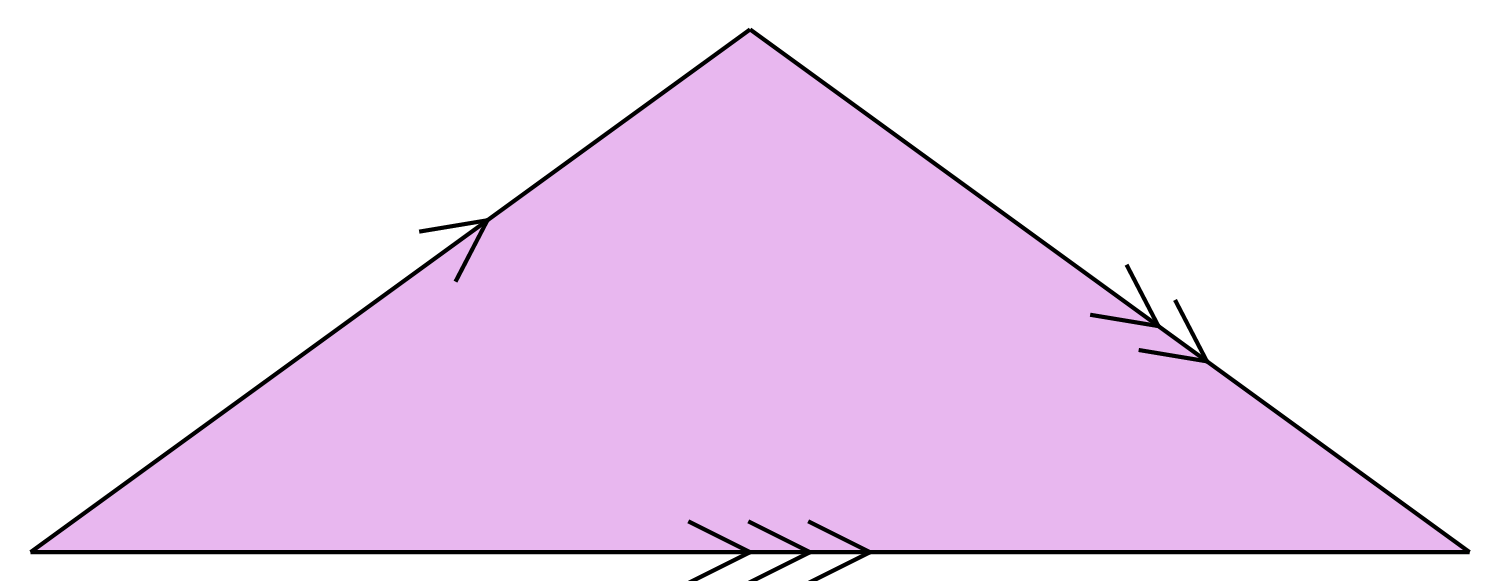
\includegraphics[width=\textwidth]{TFRob}
                \caption*{\Large T}
        \end{subfigure}\hfill
        \begin{subfigure}[t]{0.3\textwidth}
                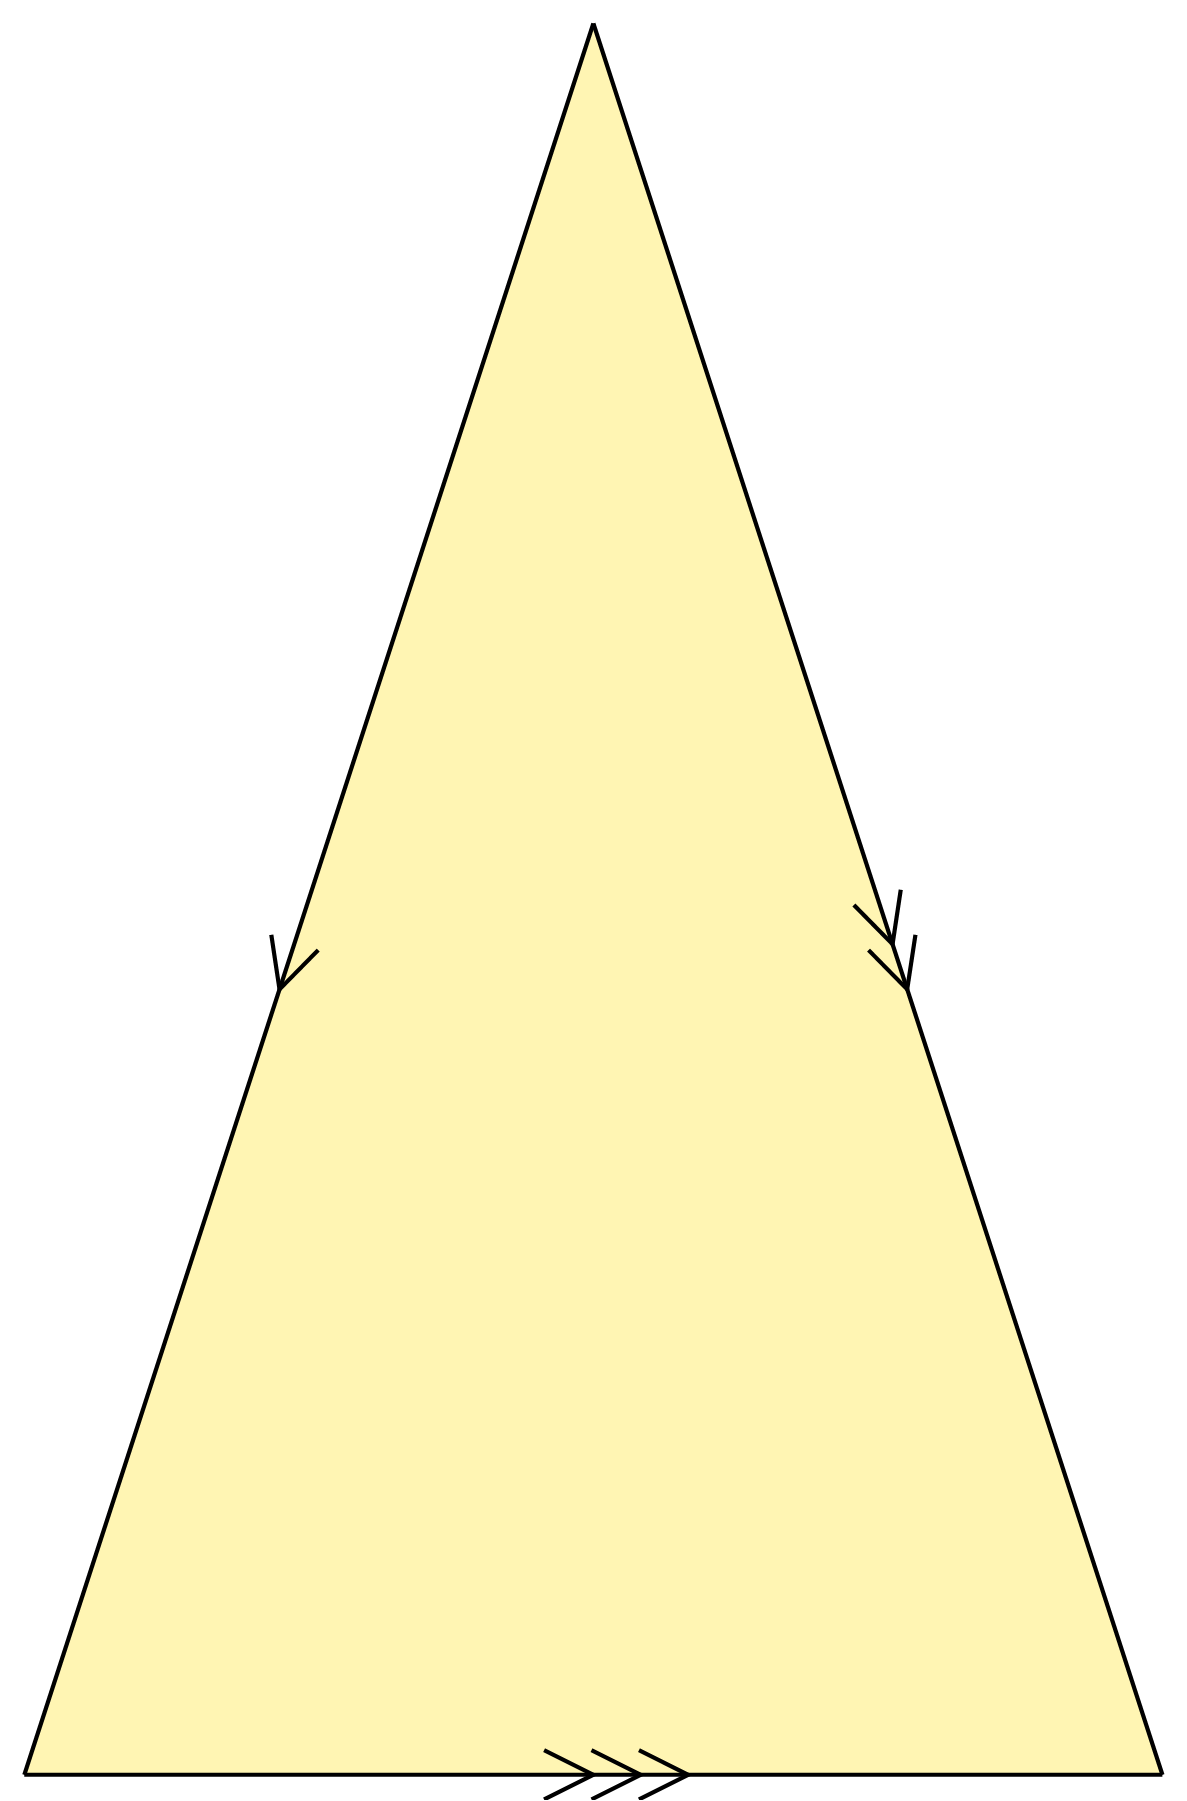
\includegraphics[width=\textwidth]{TSRob}
                \caption*{\Large t}
        \end{subfigure}\\
        
        \begin{subfigure}[t]{0.4\textwidth}
                \raisebox{0px}{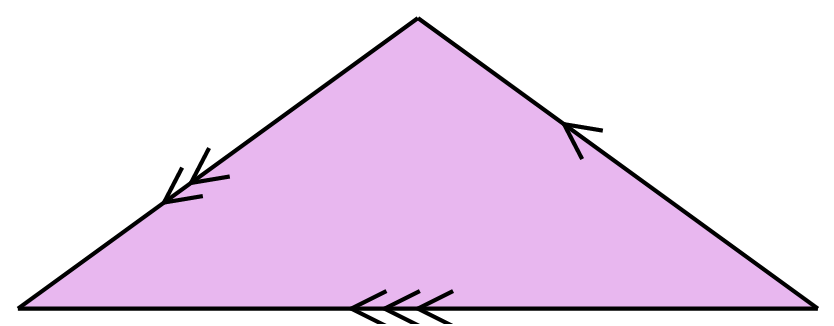
\includegraphics[width=\textwidth]{T'FRob}}
                \caption*{\Large T'}
        \end{subfigure}\hfill
        \begin{subfigure}[t]{0.3\textwidth}
                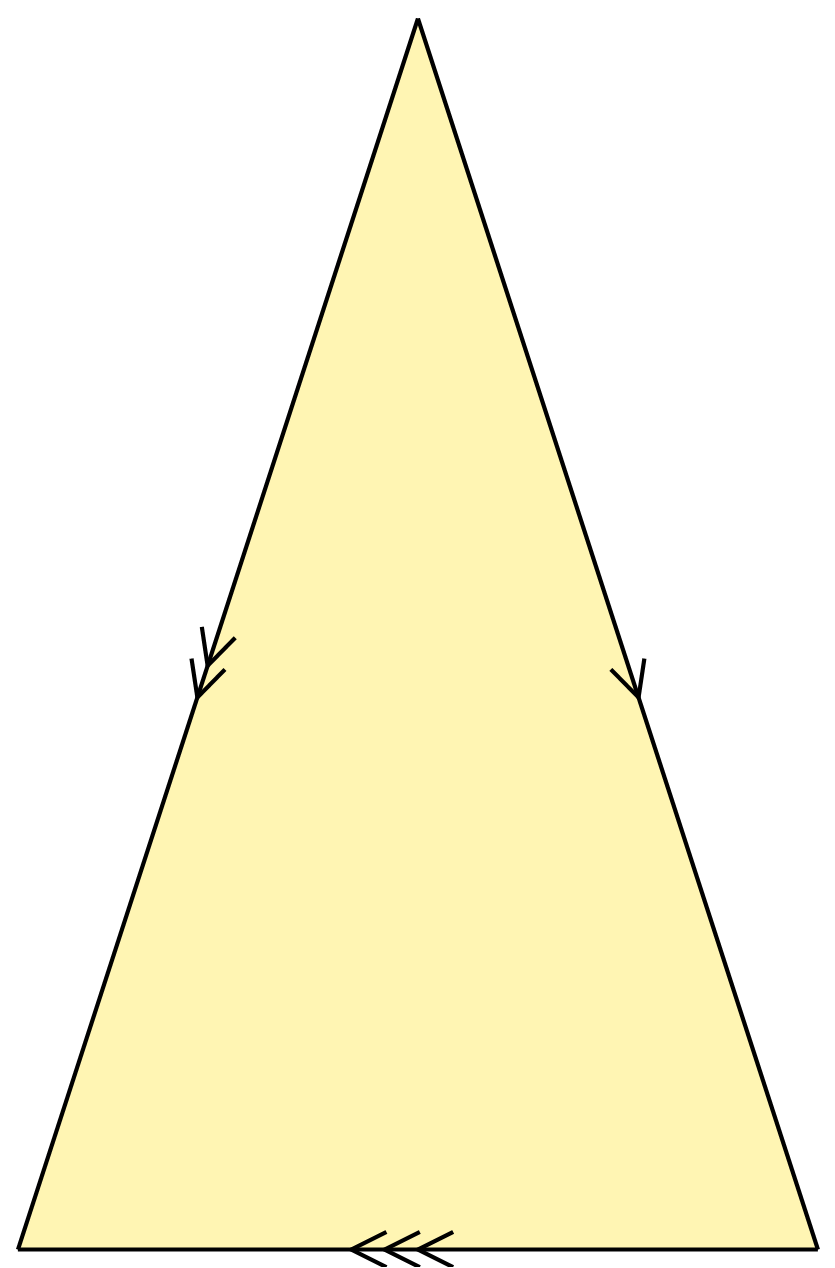
\includegraphics[width=\textwidth]{T'SRob}
                \caption*{\Large t'}
        \end{subfigure}  
        \caption{Oriented Robinson triangles. Thick or Obtuse Robinson Triangle is denoted with T. Thin or acute Robinson triangle is denoted with t. Reversed orientation is denoted with '. Arrowed edges illustrate Up-Down matching rules.}  
        \label{fig:OrientedRob}                    
\end{figure}

The matching rules under the substitution method behave slightly differently than the matching rules in the Up-Down method, illustrated with arrowed edges in Fig.\ref{fig:OrientedRob}. Here, the rules will indicate type and direction of edges, which must agree along abutting tiles. Additionally, the edge type and direction will satisfy decomposition rules according to the relationship between a triangle and it's constituent triangles, see Fig.\ref{fig:EdgeRules}. 

\begin{figure}[H]
        \begin{subfigure}[t]{0.4\textwidth}
                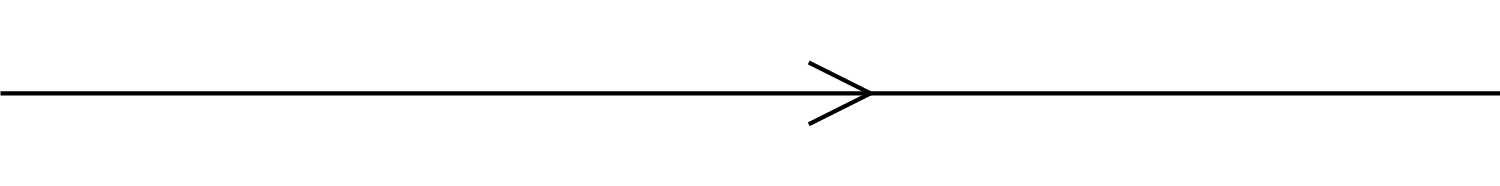
\includegraphics[width=\textwidth]{a1}
        \end{subfigure}\hfill
        \begin{subfigure}[t]{0.4\textwidth}
                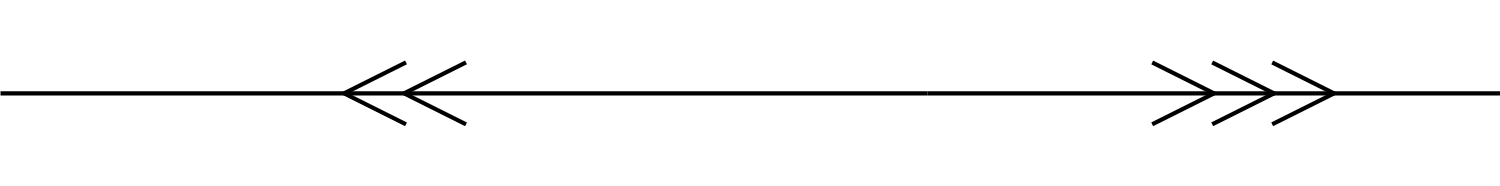
\includegraphics[width=\textwidth]{a1inflate}
        \end{subfigure}\\
        
        \begin{subfigure}[t]{0.4\textwidth}
                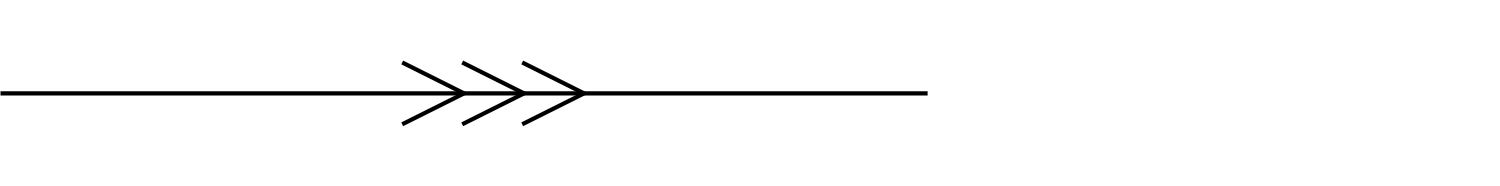
\includegraphics[width=\textwidth]{a2}
        \end{subfigure}\hfill
        \begin{subfigure}[t]{0.4\textwidth}
                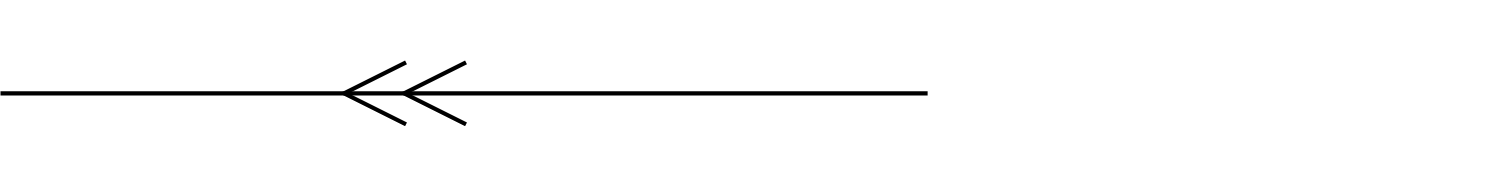
\includegraphics[width=\textwidth]{a2inflate}
        \end{subfigure}\\    
        
        \begin{subfigure}[t]{0.4\textwidth}
                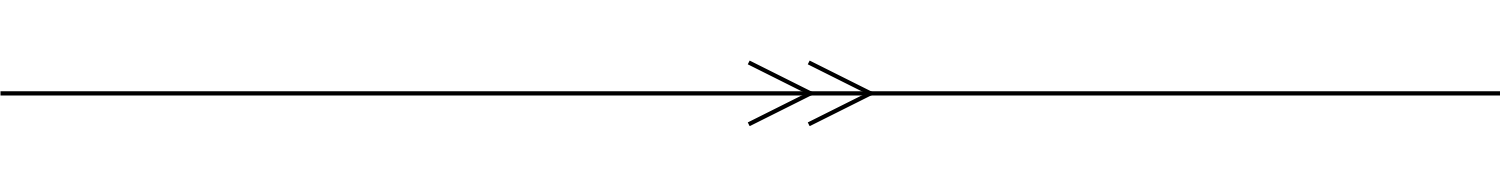
\includegraphics[width=\textwidth]{a3}
        \end{subfigure}\hfill
        \begin{subfigure}[t]{0.4\textwidth}
                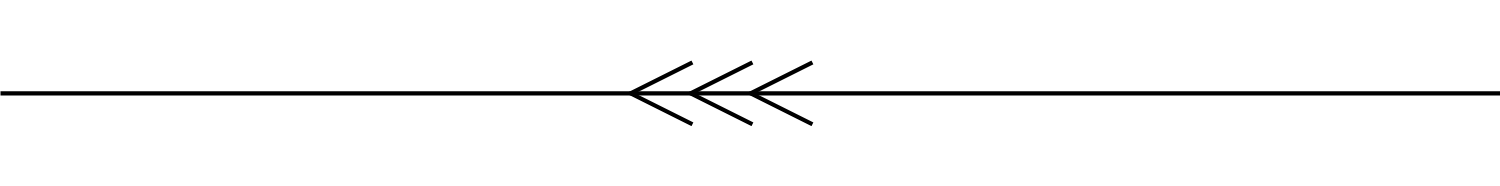
\includegraphics[width=\textwidth]{a3inflate}
        \end{subfigure}\\                           
        
        \begin{subfigure}[t]{0.4\textwidth}
                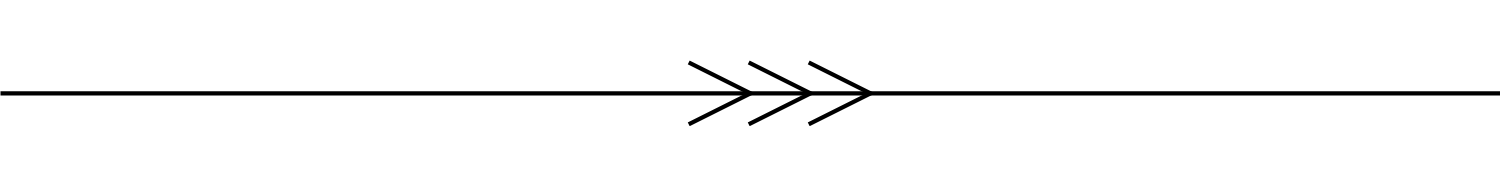
\includegraphics[width=\textwidth]{a4}
        \end{subfigure}\hfill
        \begin{subfigure}[t]{0.4\textwidth}
                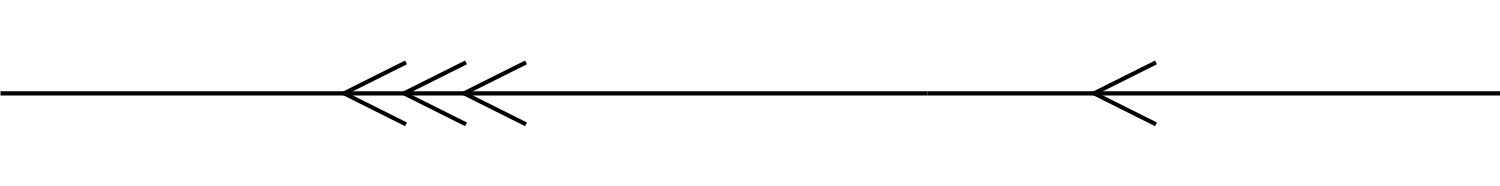
\includegraphics[width=\textwidth]{a4inflate}
        \end{subfigure}\\   
        \caption{Parent edges (Left) and their constituent edges (Right)}     
        \label{fig:EdgeRules}
\end{figure} 


\pagebreak
Consider again the substitution rules on the Robinson triangles described in Fig.\ref{fig:RobSubs}. This substitution is also employed in the Up-Down method. However, in this case we will label the constituent triangles of the substitution. We do this so we can explicitly describe the relationship between a constituent triangle and its parent triangle. We label this relationship using mapping functions, given by lowercase Greek letters: $\alpha, \beta, \delta, \gamma$. We see the oriented Robinson triangles, substituted with relationship labels, in Fig.\ref{fig:OrientedSub}.

These relationship labels can be considered as mappings from a constituent triangle to its parent triangle. These mappings are as follows:
\begin{align}
\epsilon &: T \rightarrow T  &\epsilon' &: T' \rightarrow T' \nonumber\\  
\alpha &: T \rightarrow t  &\alpha' &: T' \rightarrow t' \nonumber\\  
\beta &: t \rightarrow t  &\beta' &: t' \rightarrow t' \label{eq:maps}\\  
\delta &: t' \rightarrow T  &\delta' &: t \rightarrow T' \nonumber\\ 
\gamma &: T' \rightarrow T  &\gamma' &: T \rightarrow T' \nonumber
\end{align}
Again, these mappings are also labeled in Fig.\ref{fig:OrientedSub}. For an example of how to interpret this mapping, consider the mapping $\delta$ which maps constituent \textbf{t'} to parent \textbf{T}. This tells us that following relationship $\delta$, the yellow \textbf{t'} triangle will be located inside the pink \textbf{T} parent.



\begin{figure}[H]
        \begin{subfigure}[t]{0.55\textwidth}
                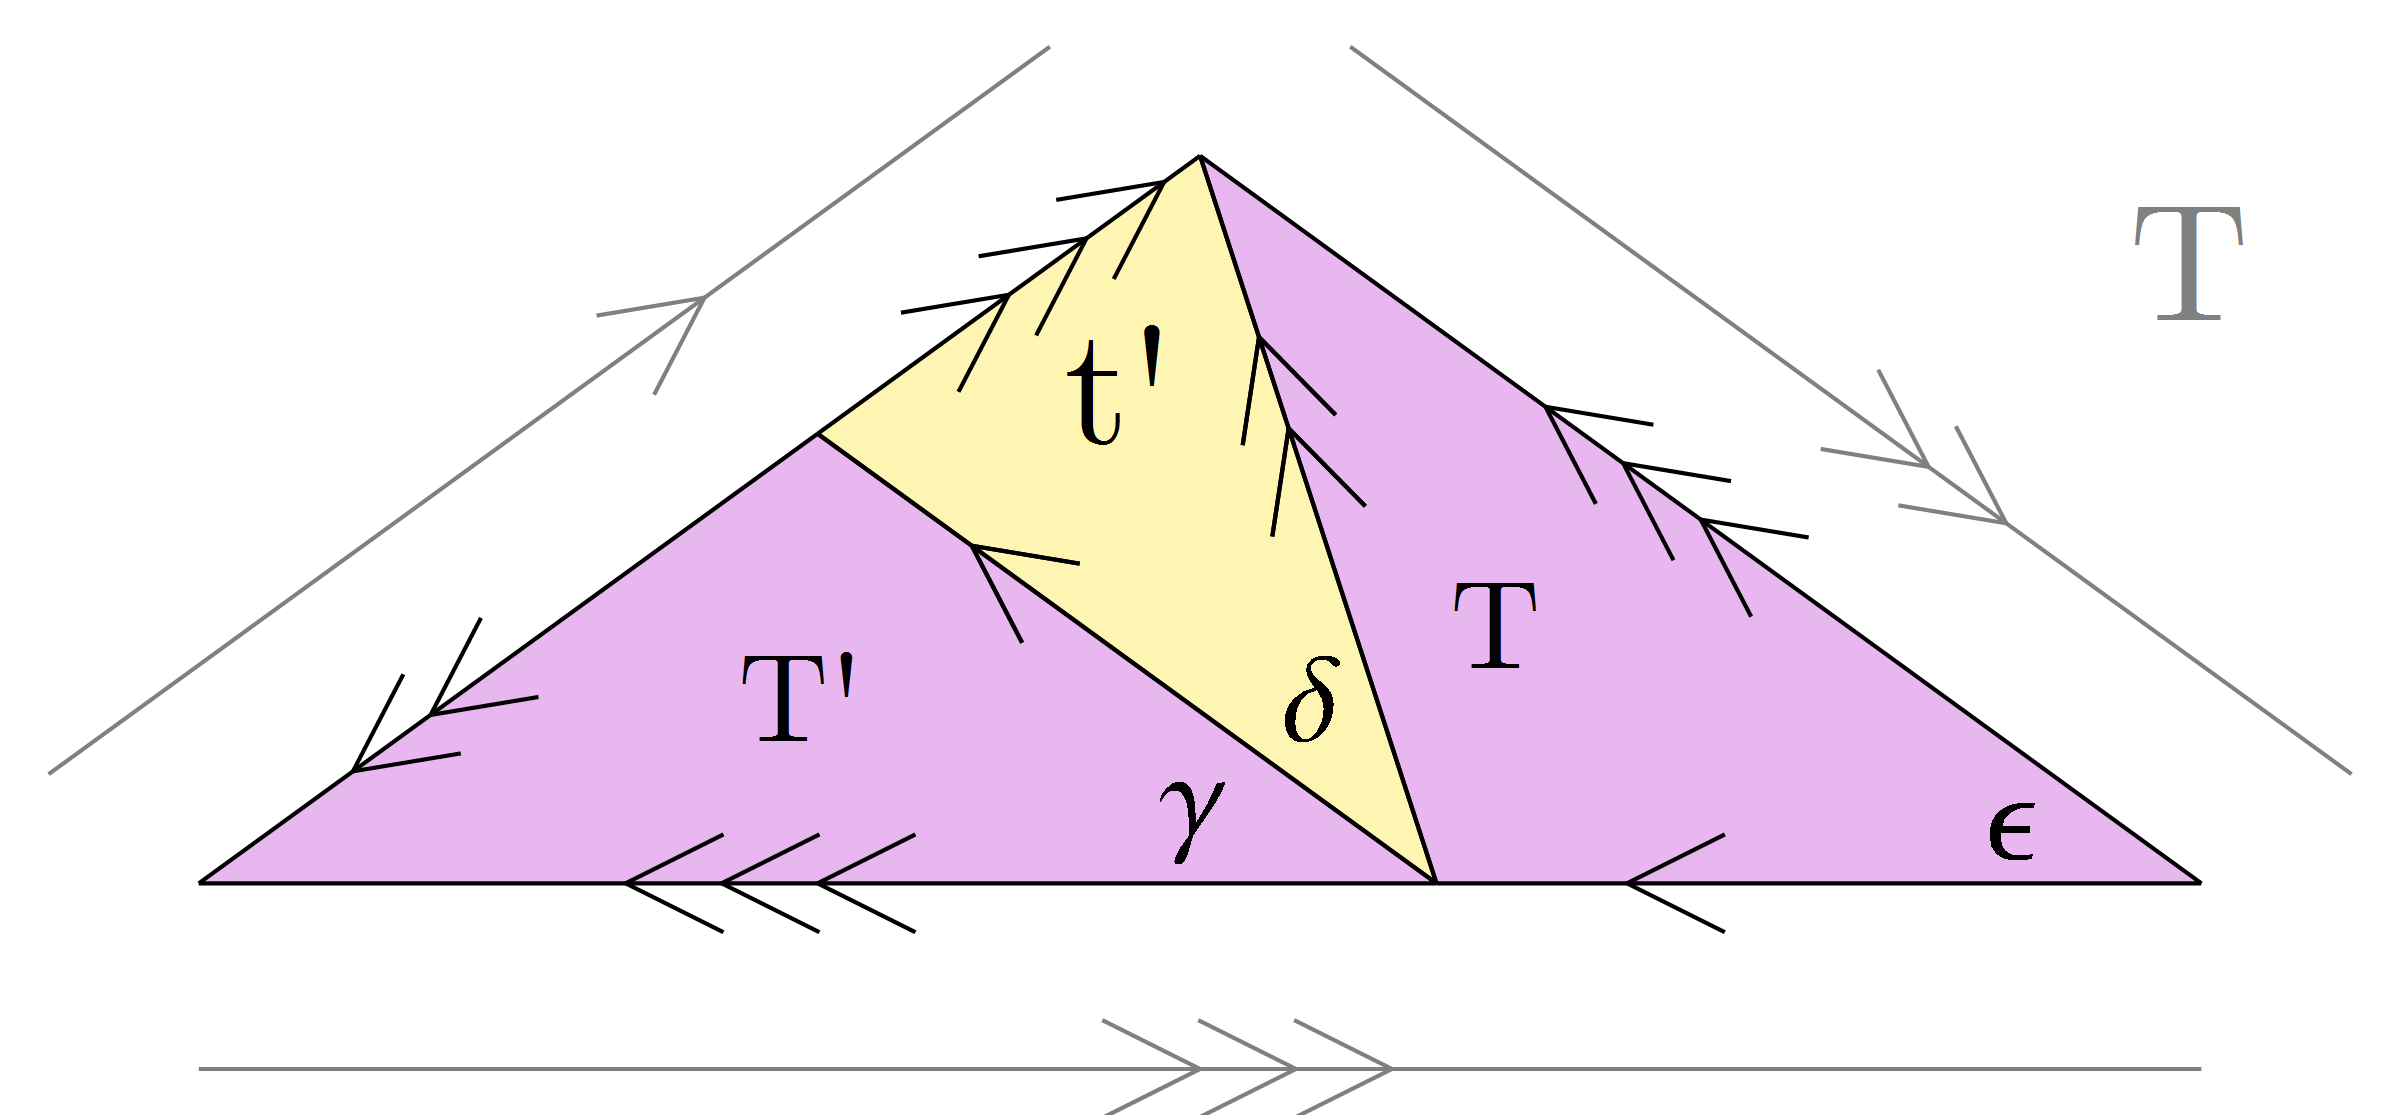
\includegraphics[width=\textwidth]{TF}
        \end{subfigure}\hfill
        \begin{subfigure}[t]{0.35\textwidth}
                \includegraphics[width=\textwidth]{TS}
        \end{subfigure}\\
        
        \begin{subfigure}[t]{0.55\textwidth}
                \raisebox{55px}{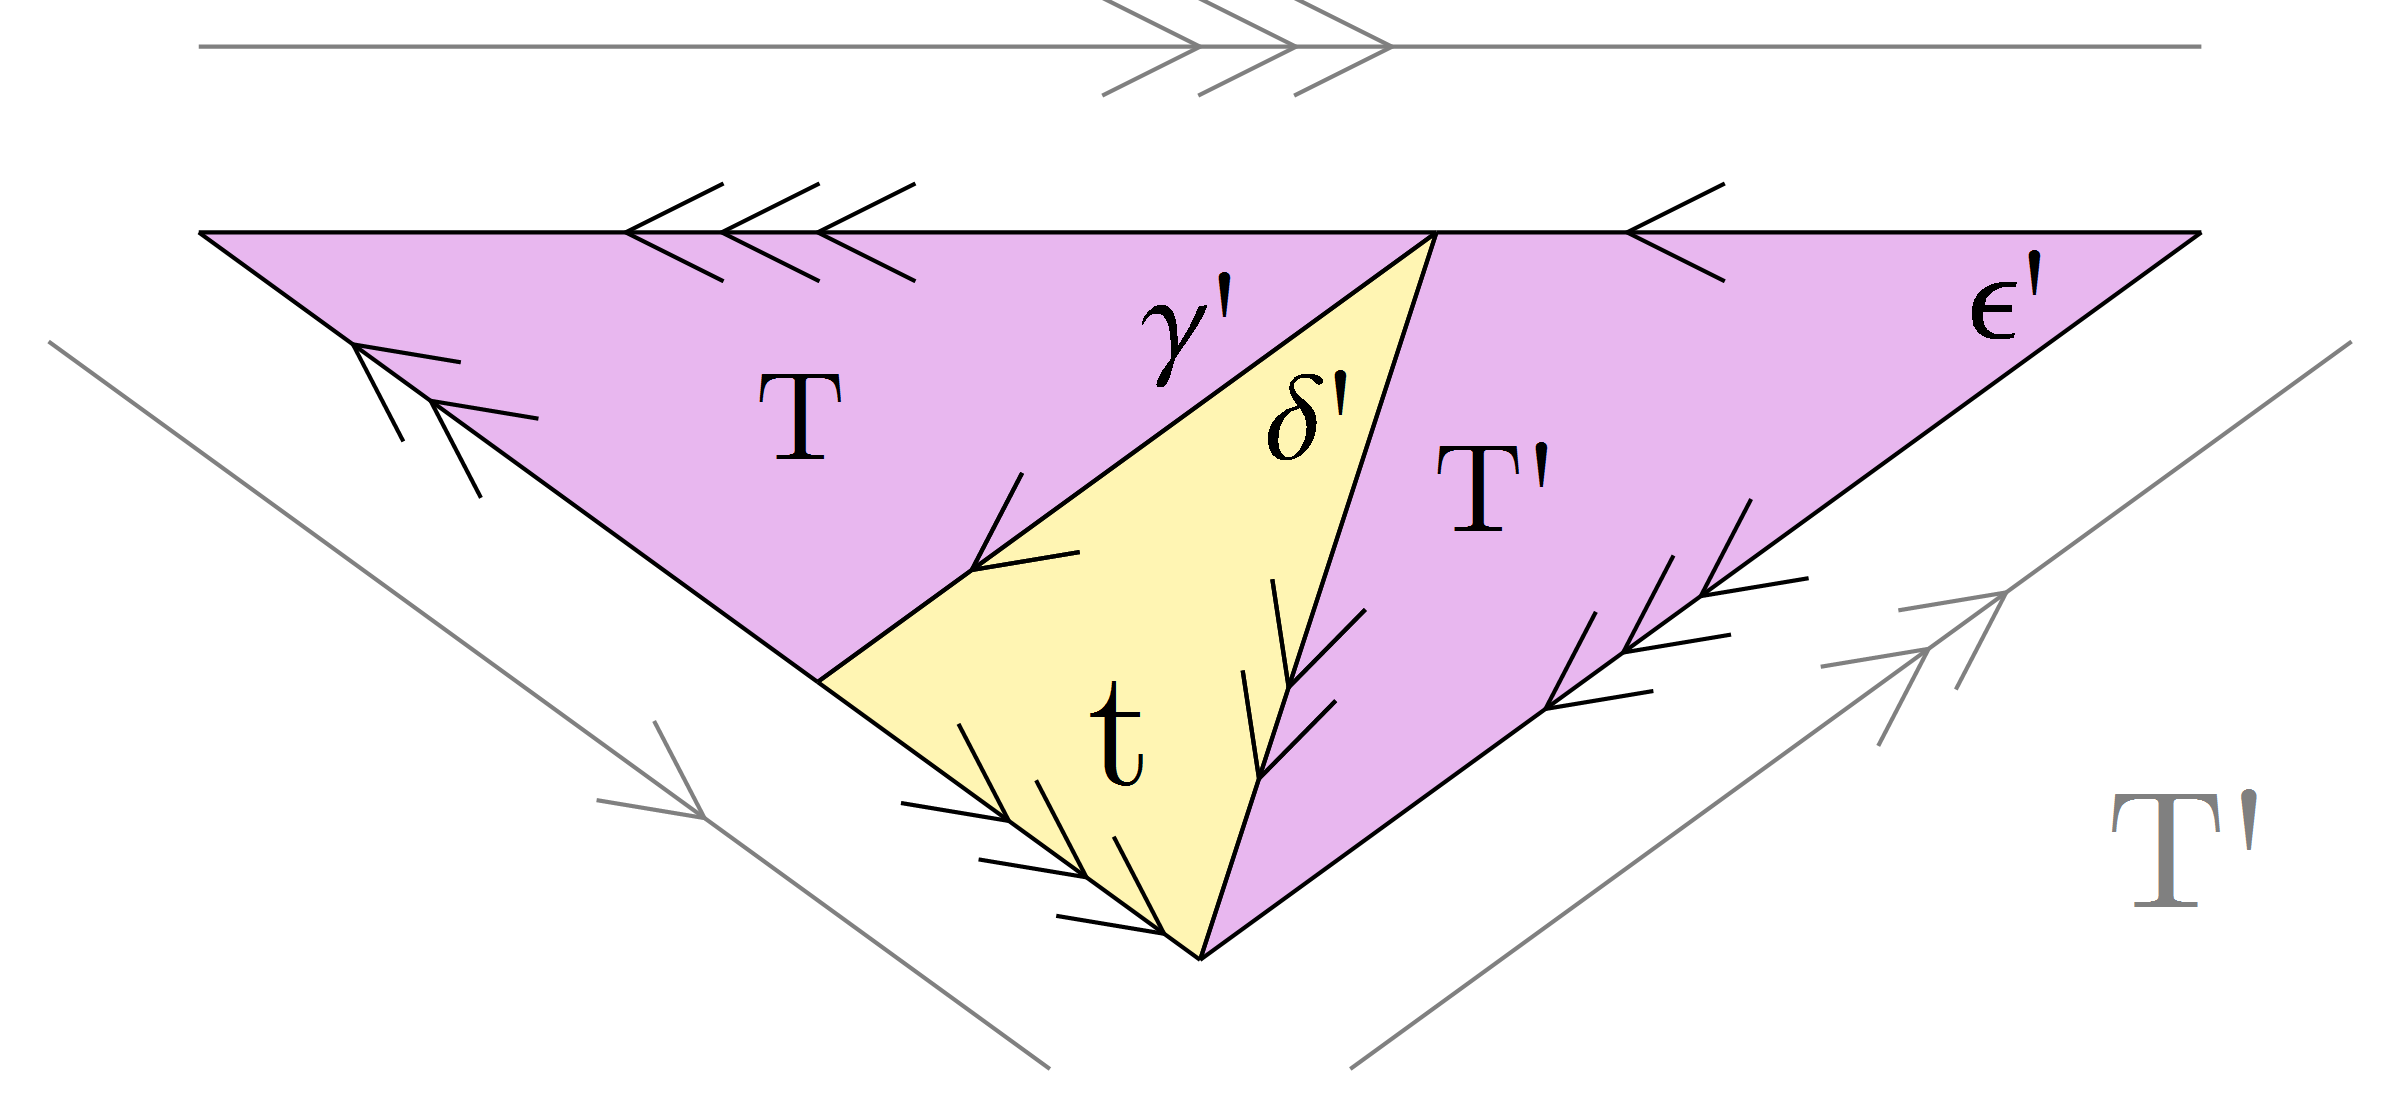
\includegraphics[width=\textwidth]{TF'}}
        \end{subfigure}\hfill
        \begin{subfigure}[t]{0.35\textwidth}
                \includegraphics[width=\textwidth]{TS'}
        \end{subfigure}   
        \caption{Oriented Robinson triangles with their constituent triangles. The relationship mappings between a constituent and parent triangles are given by lowercase Greek letters. For example, constituent triangle \textbf{T'} is related to parent triangle \textbf{T} under the mapping $\gamma$. The original edges of the parent triangles are also shown in grey. The relationship between the constituent and parent edges is shown in Fig.\ref{fig:EdgeRules}.}
        \label{fig:OrientedSub}                     
\end{figure}

From these mappings we can see why the explicit description of triangle orientation is necessary here. Otherwise, for instance, it would be ambiguous which constituent thick triangle, \textbf{T} or \textbf{T'}, we are describing inside a parent \textbf{T}.

We can alternatively visualize the mappings in Equations (\ref{eq:maps}) as directed graphs embedding constituent triangles into parent triangles, see Fig.\ref{fig:functionmap}. 

\begin{figure}[H]
        \begin{subfigure}[t]{0.6\textwidth}
                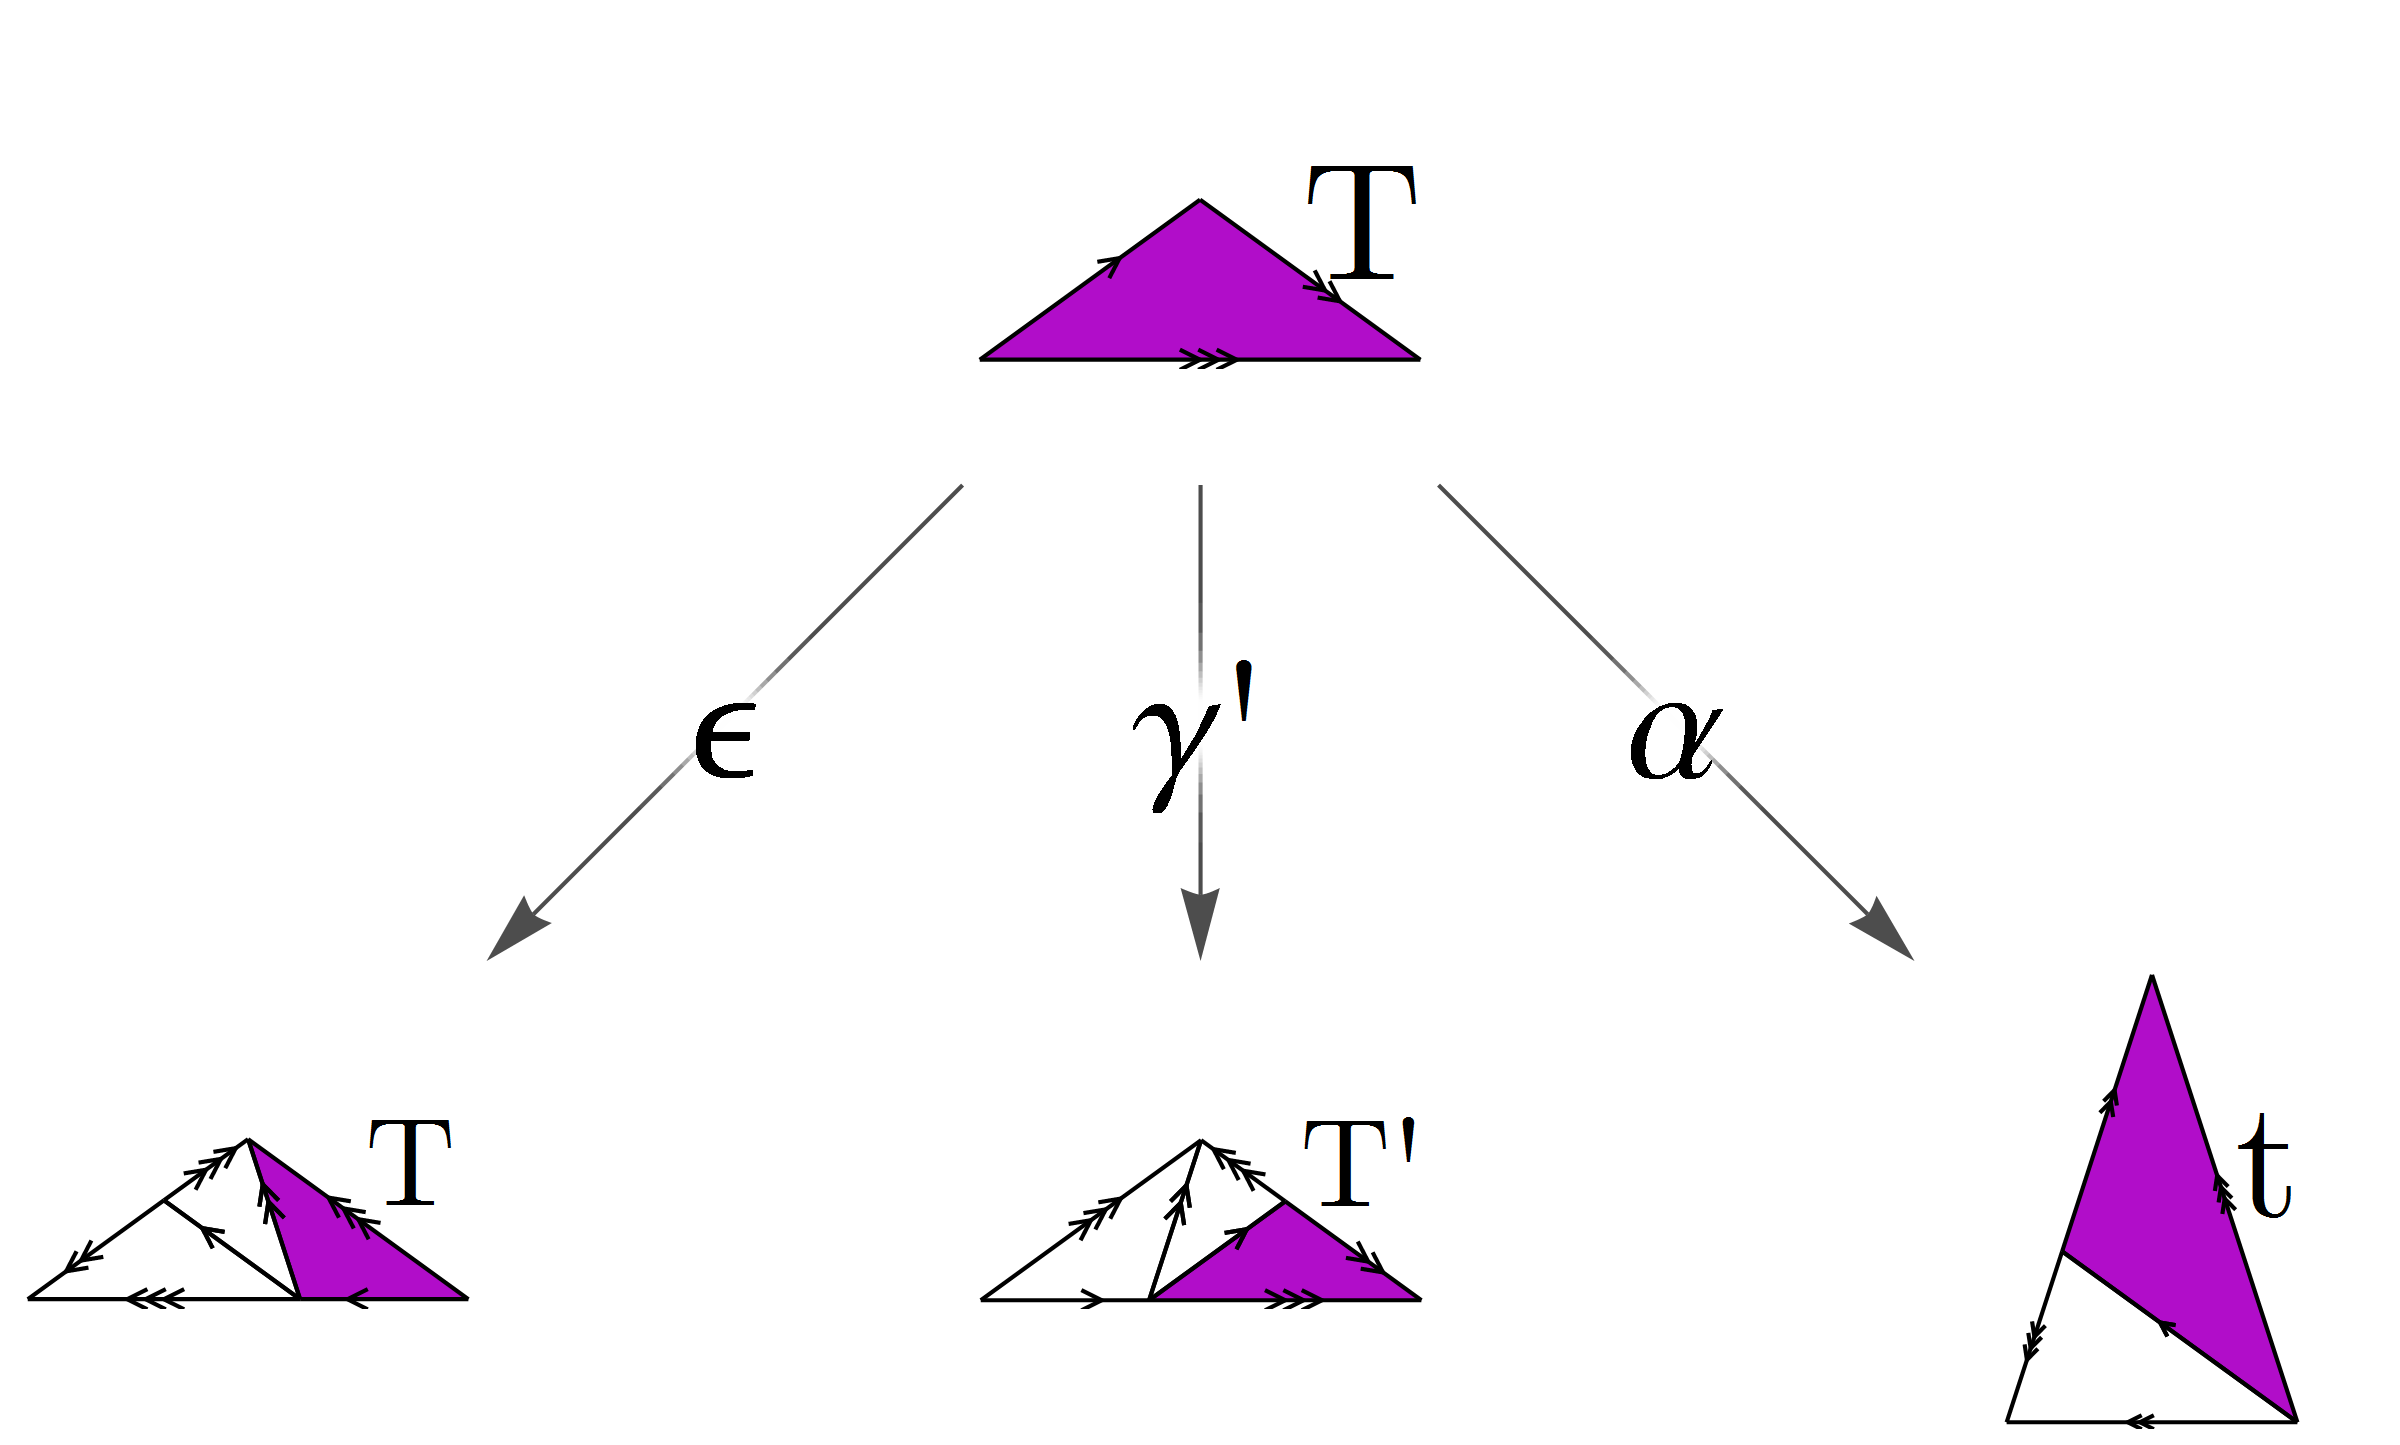
\includegraphics[width=\textwidth]{TRgraph}
        \end{subfigure}\hfill
        \begin{subfigure}[t]{0.4\textwidth}
                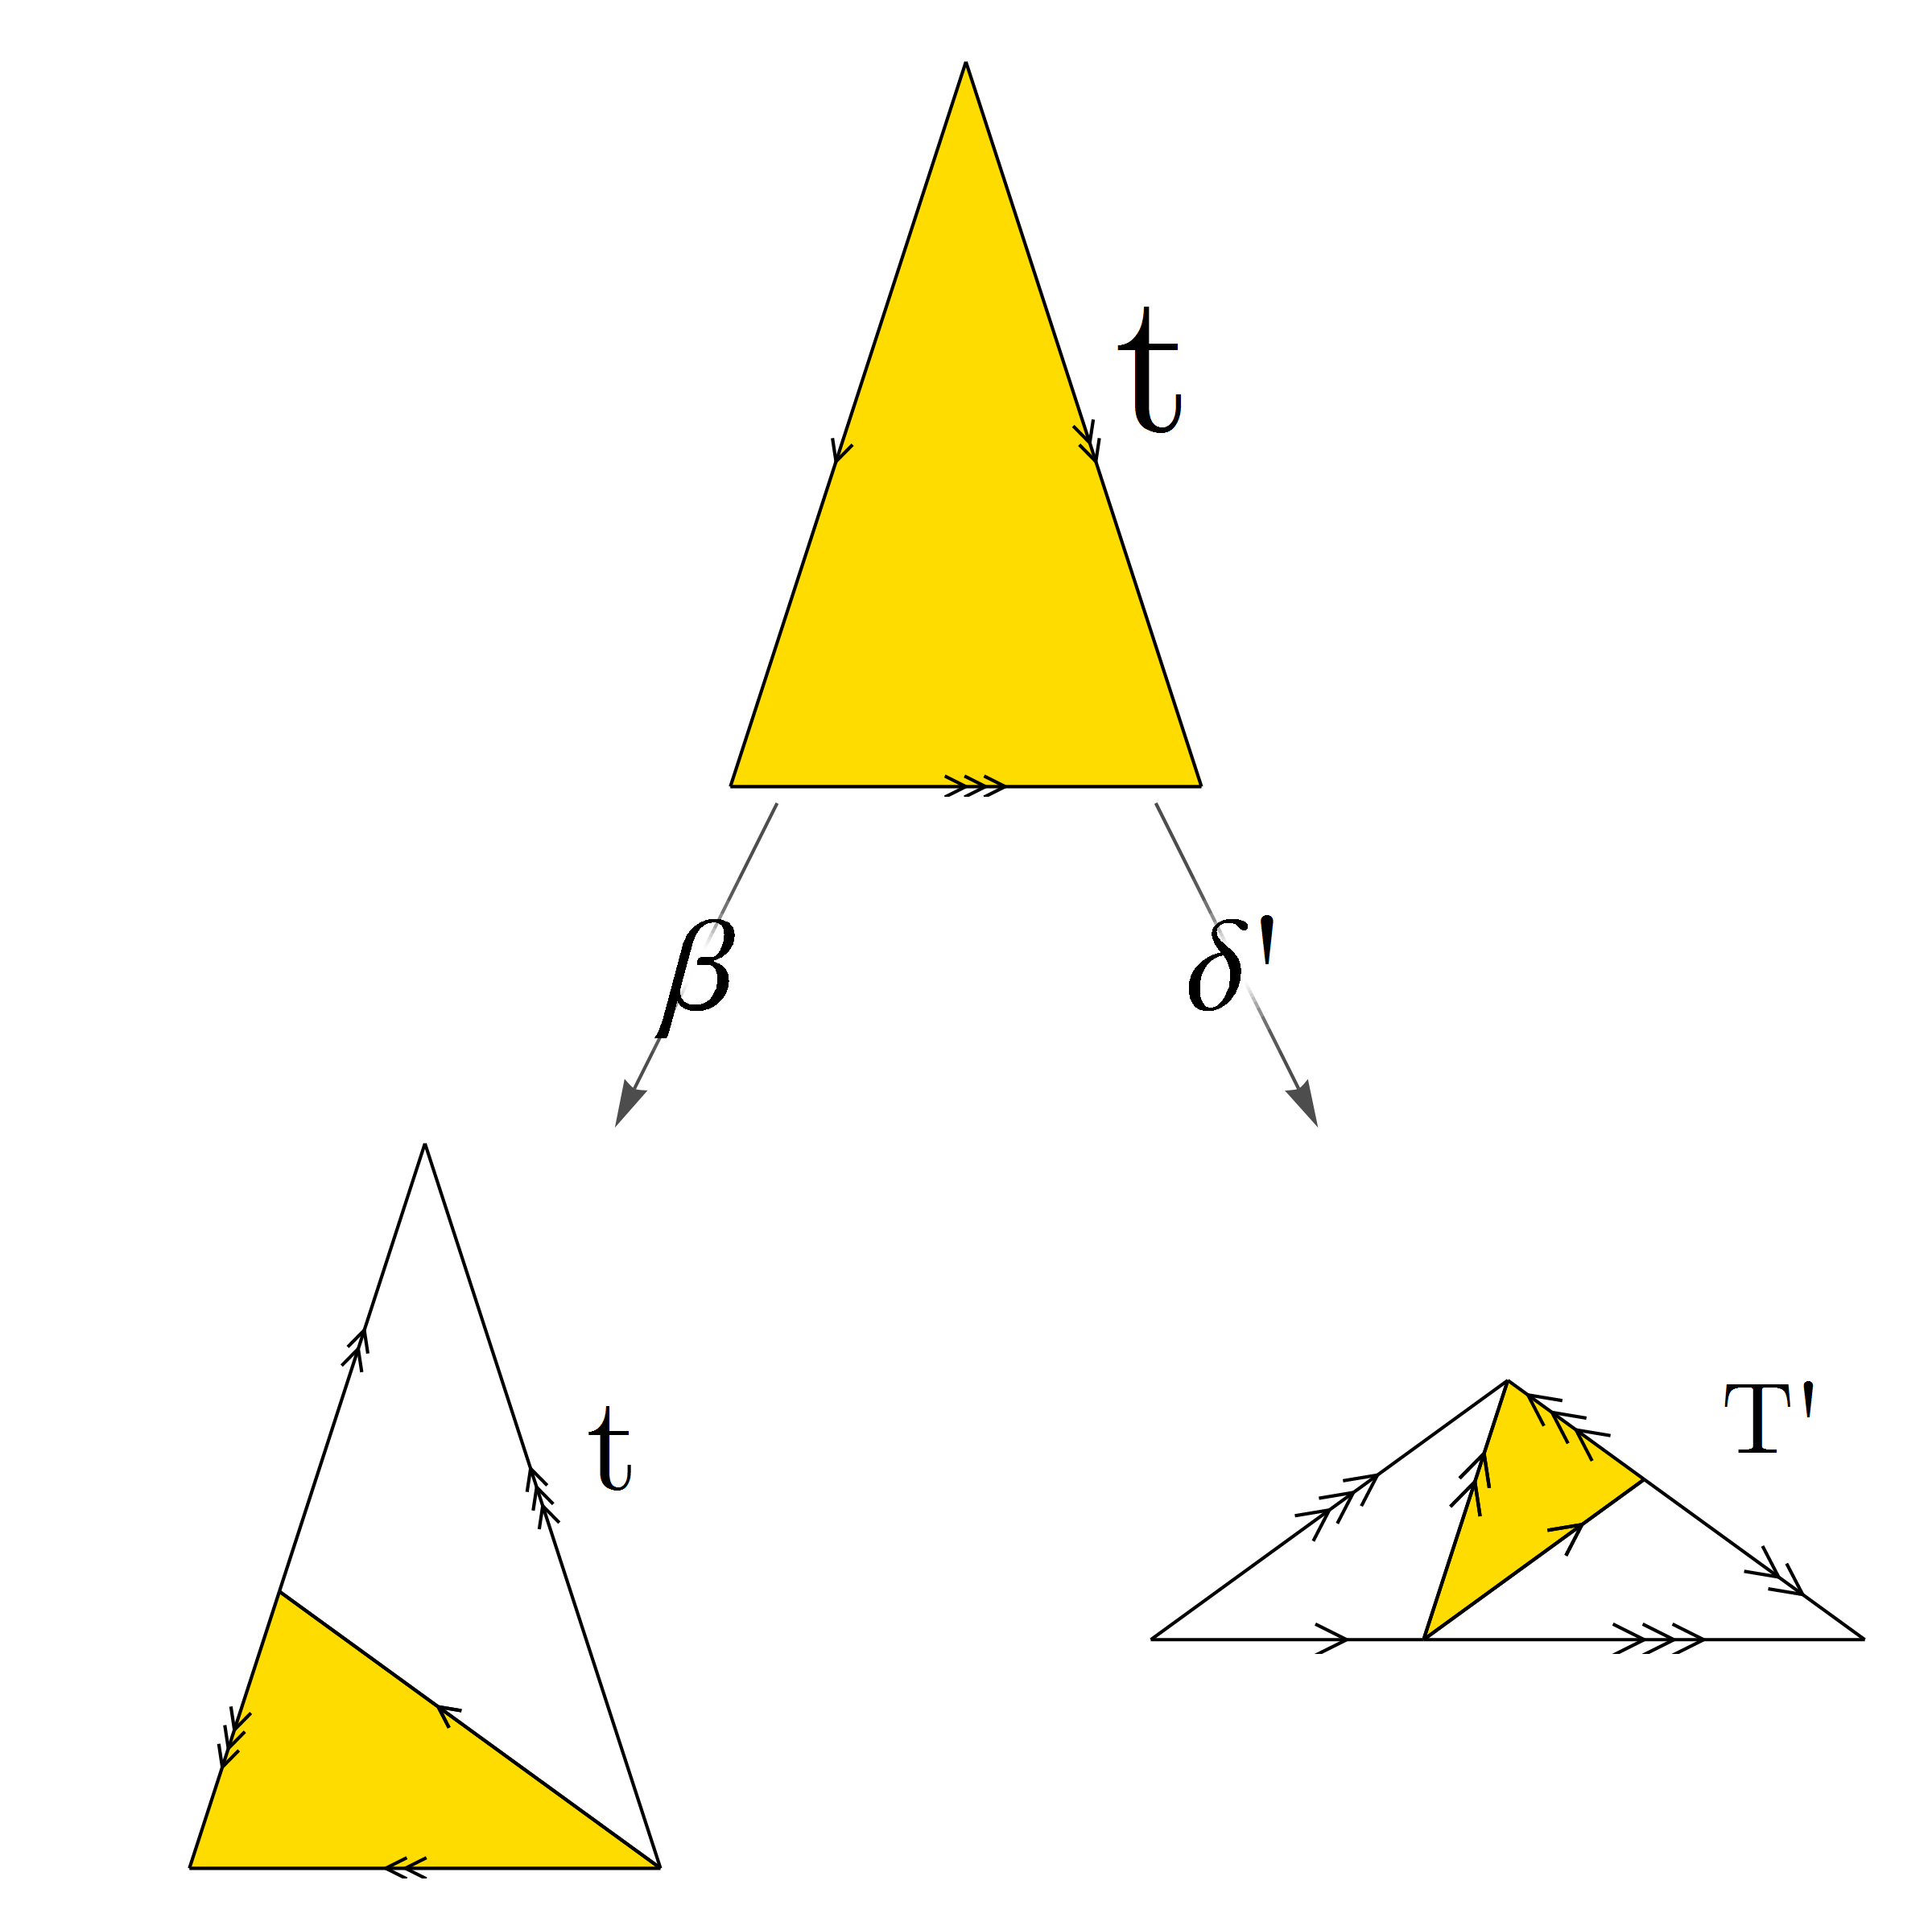
\includegraphics[width=\textwidth]{tsrgraph}
        \end{subfigure}\\
        
        \begin{subfigure}[t]{0.6\textwidth}
                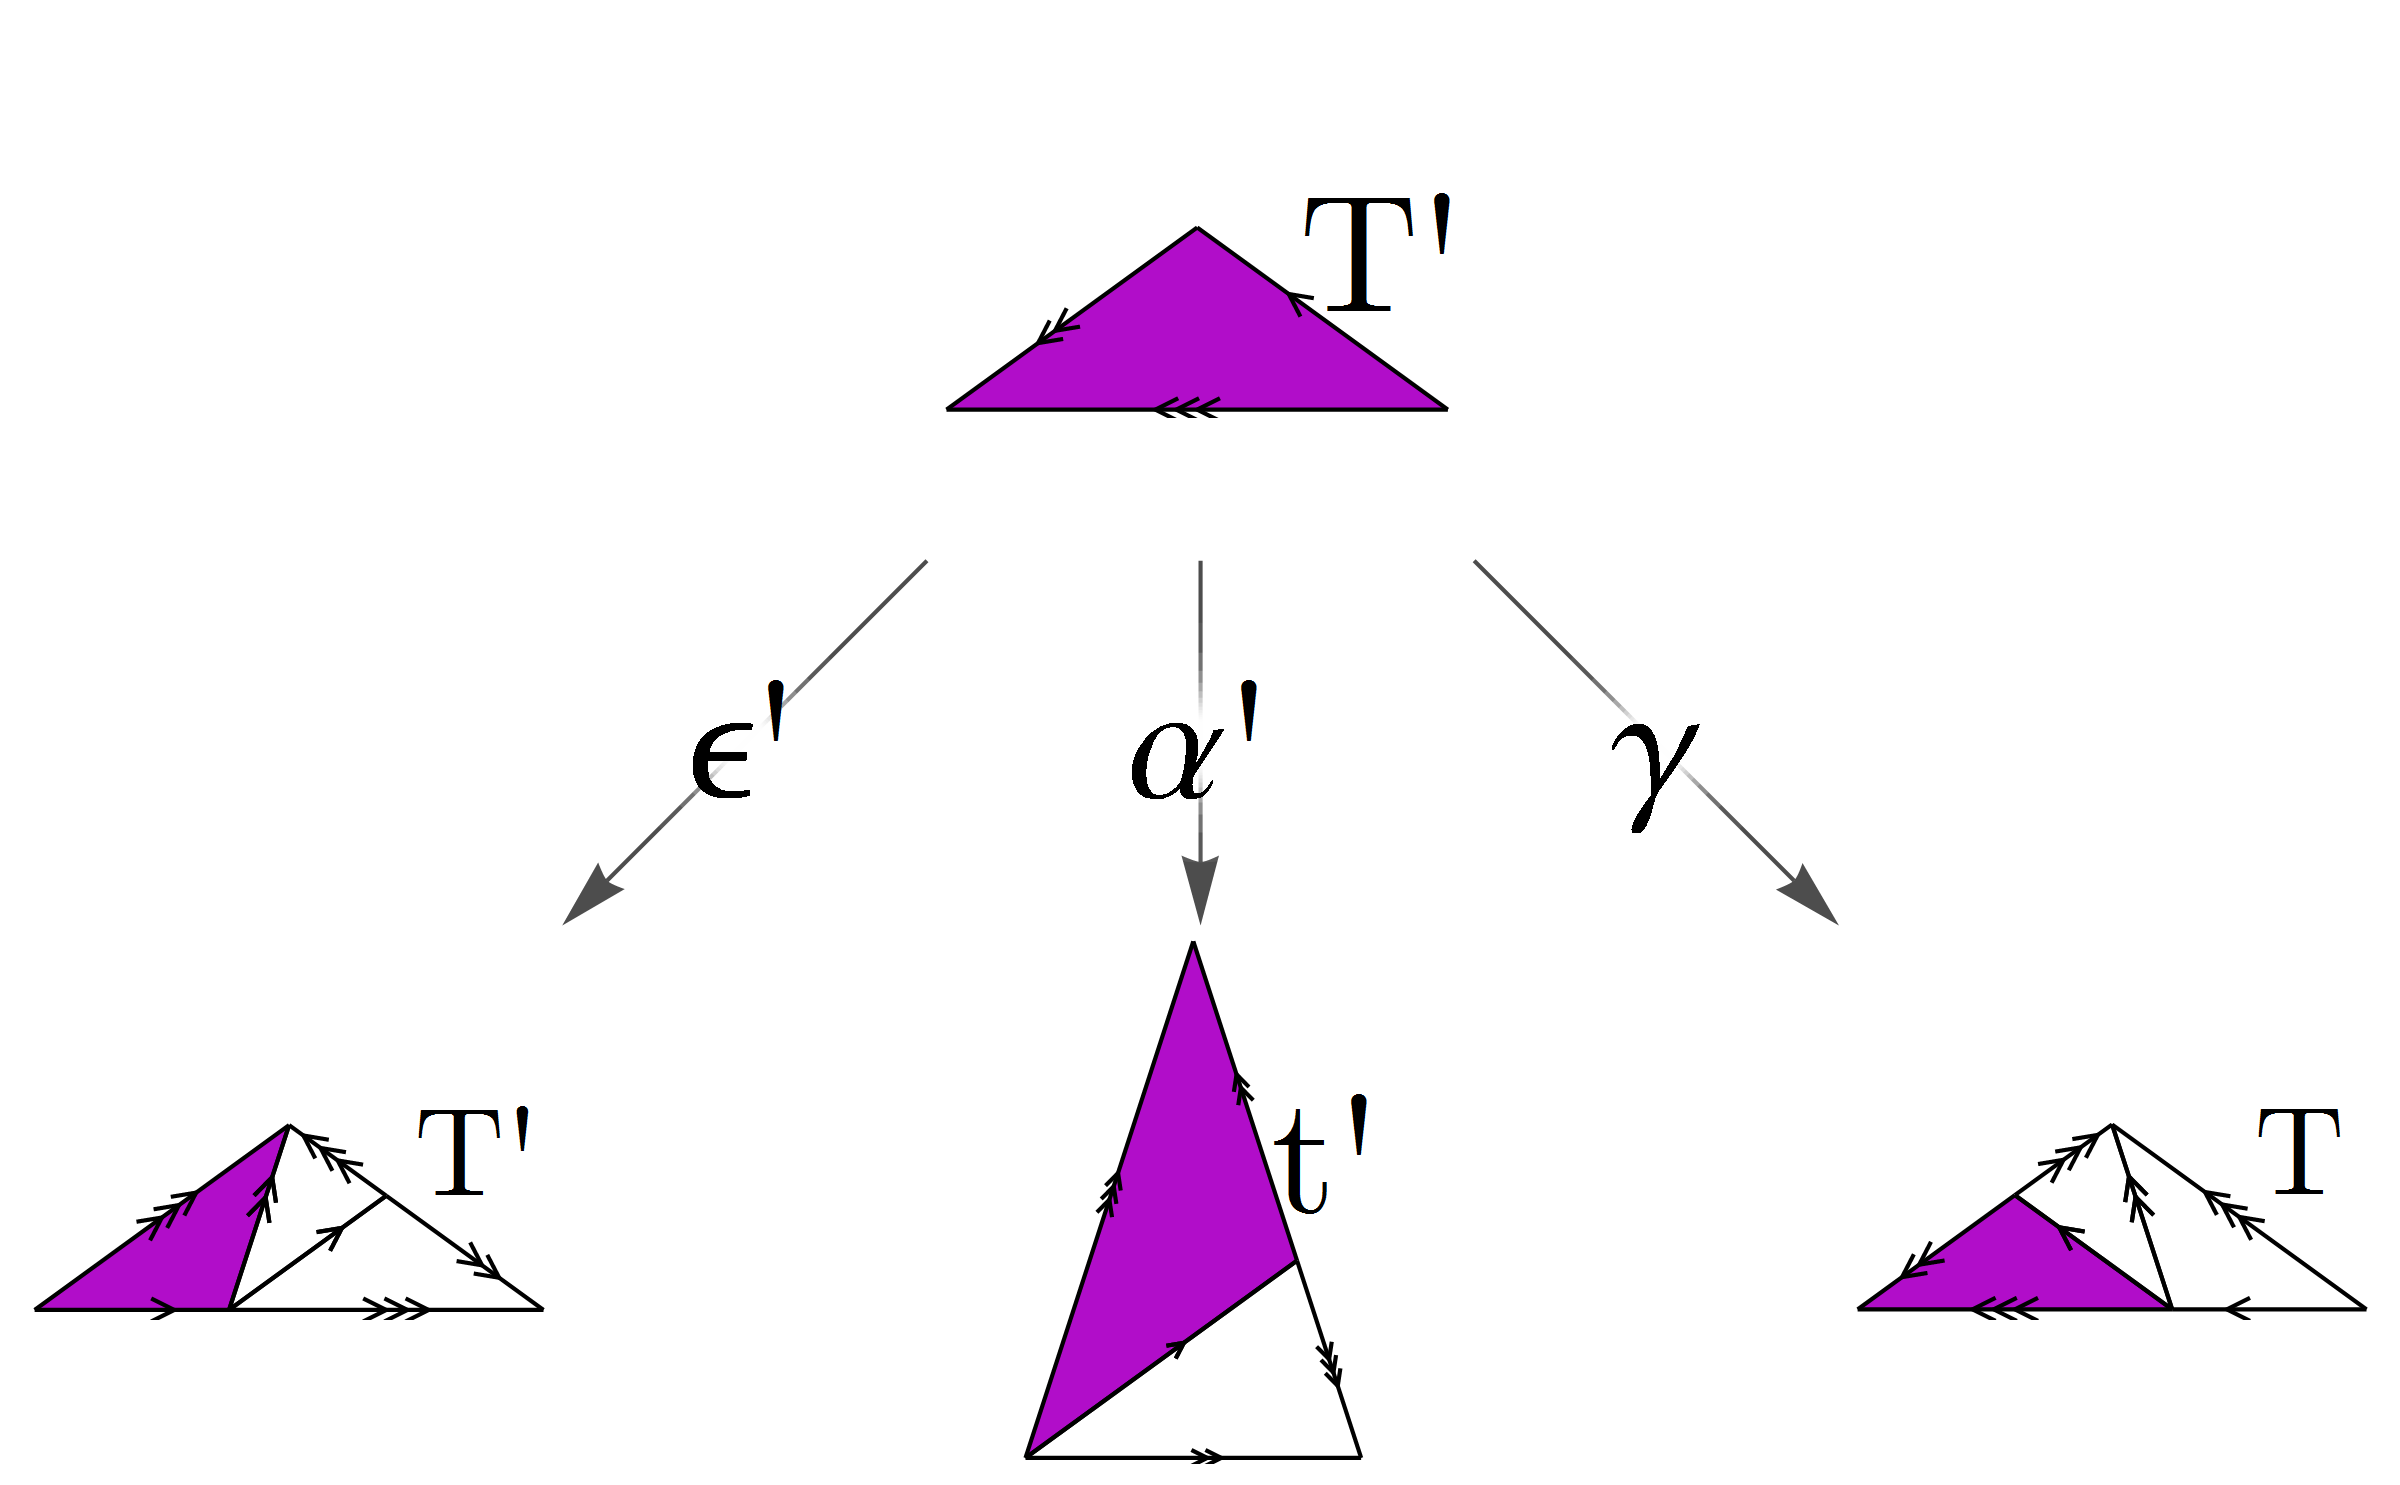
\includegraphics[width=\textwidth]{TLgraph}
        \end{subfigure}\hfill
        \begin{subfigure}[t]{0.4\textwidth}
                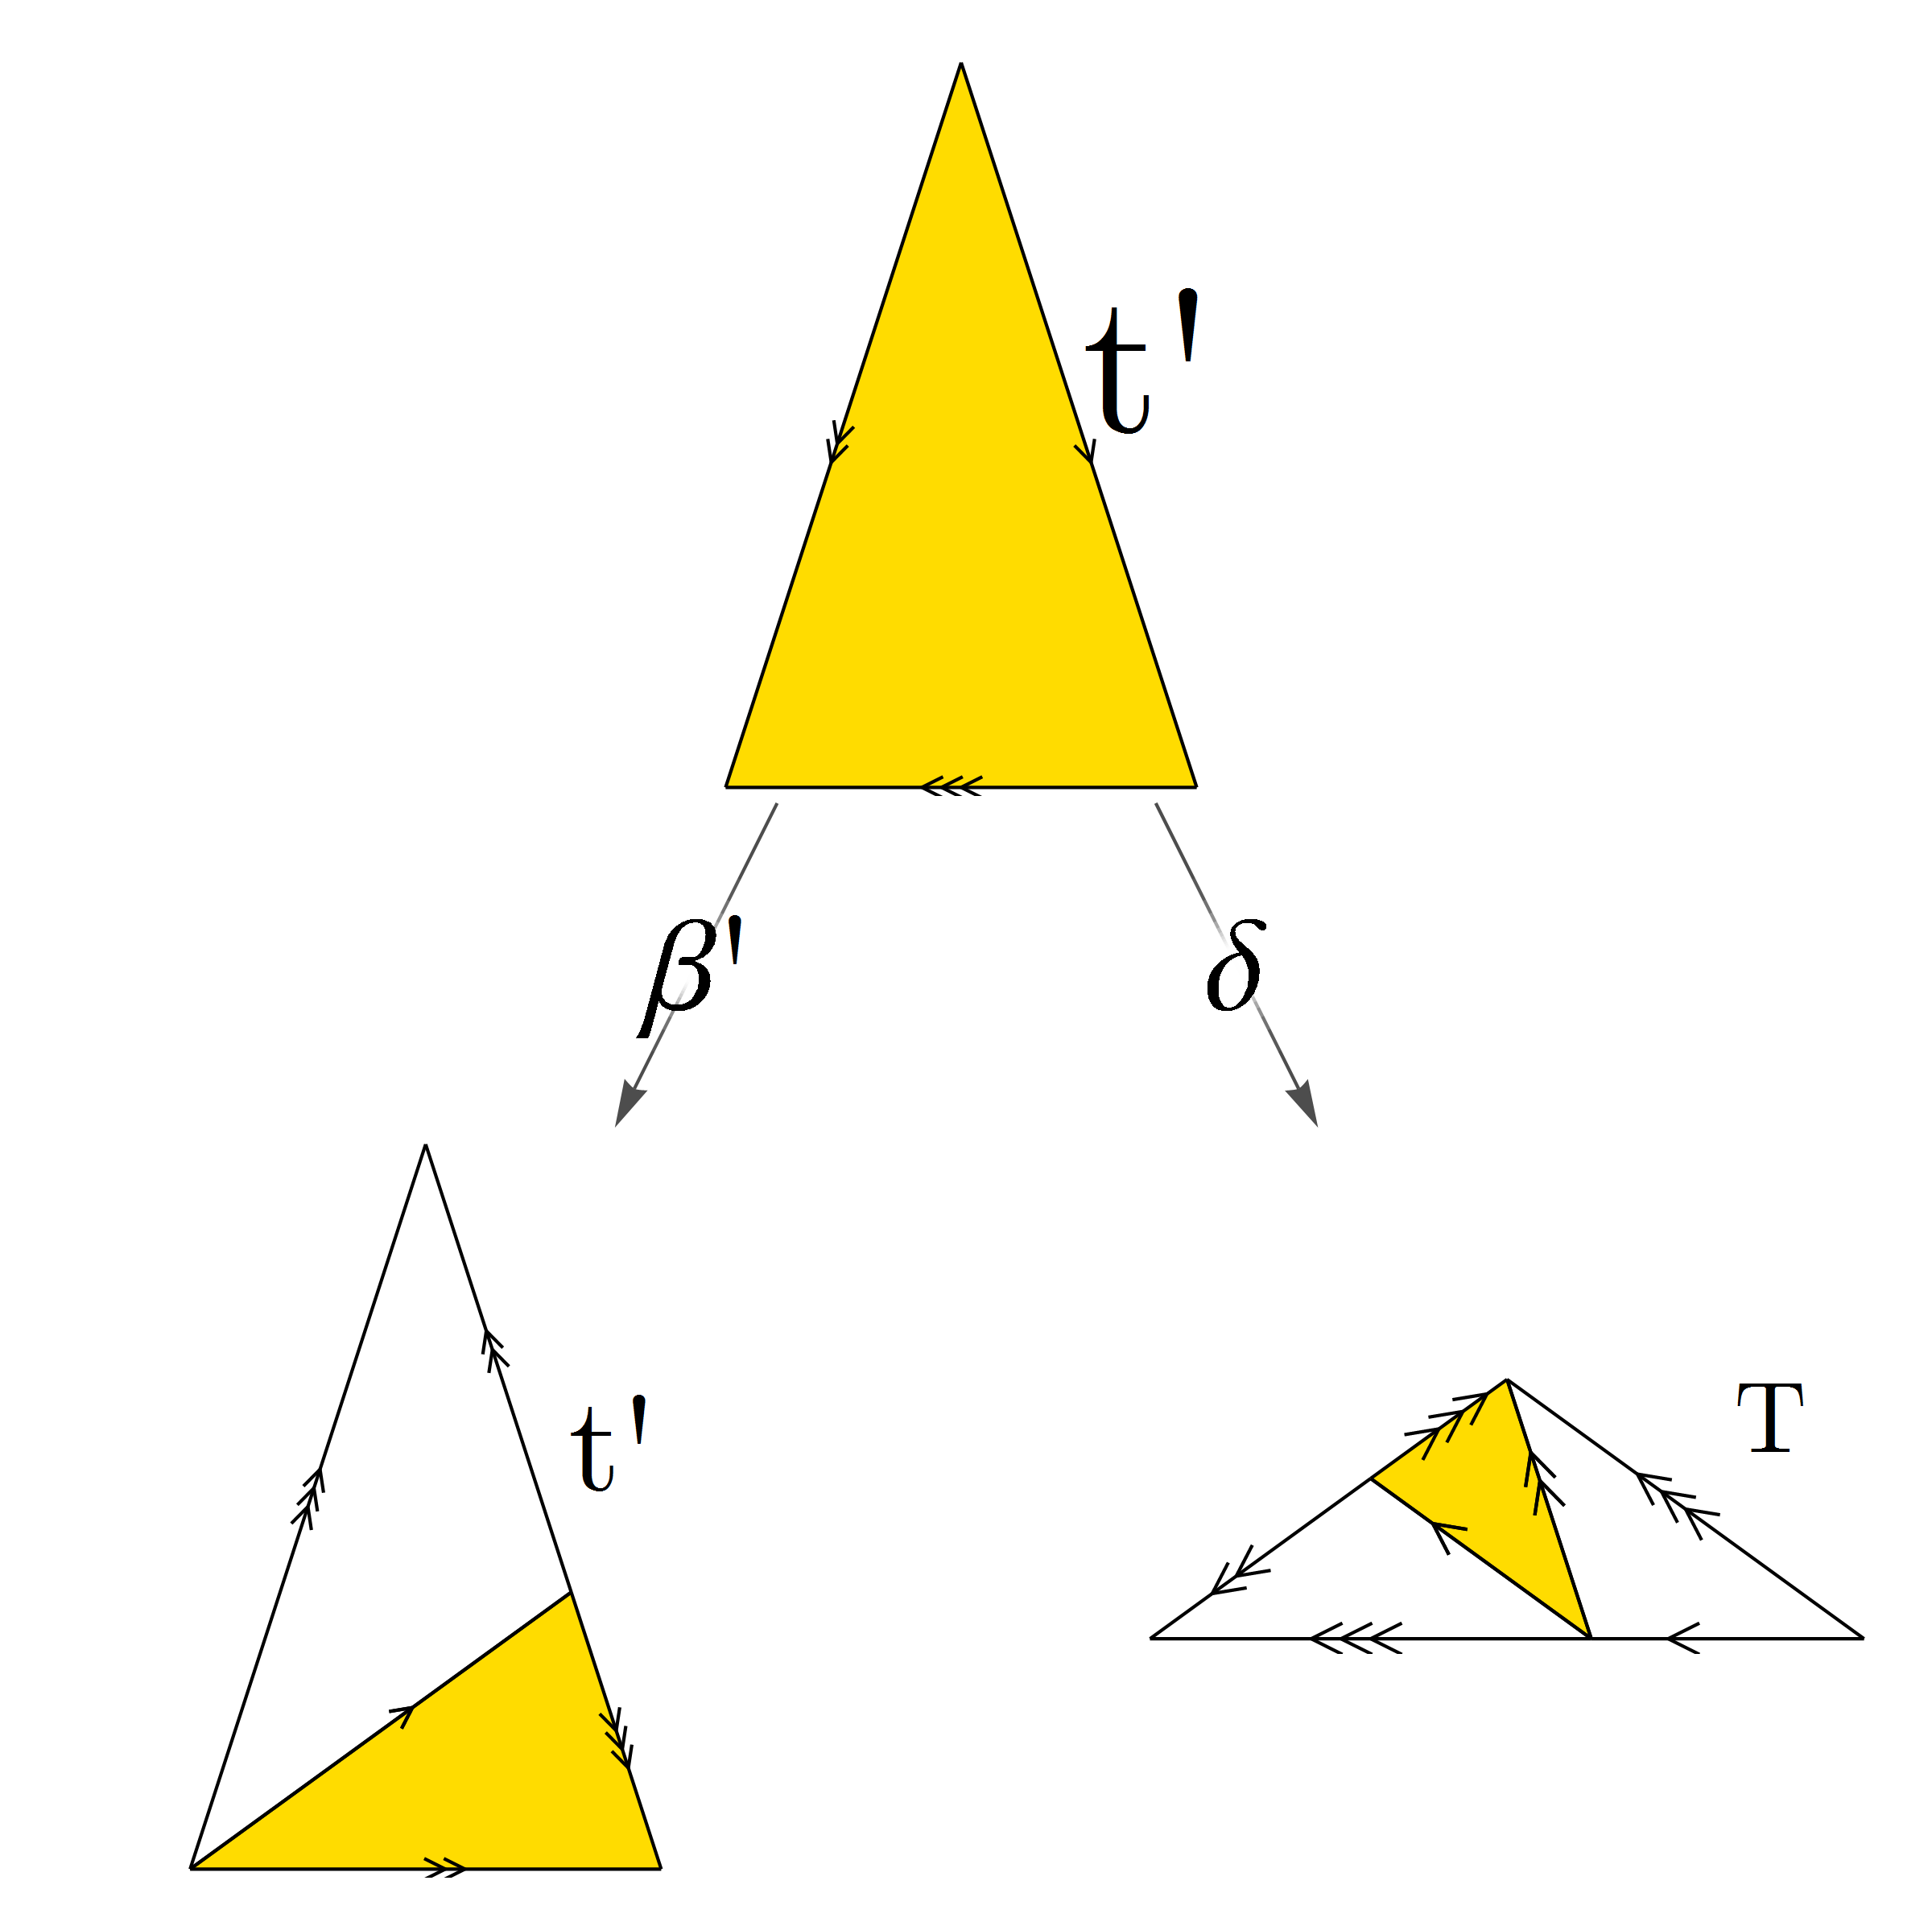
\includegraphics[width=\textwidth]{tslgraph}
        \end{subfigure}  
        \caption{Relationship mapping from constituent triangles to parent triangles given by Equations (\ref{eq:maps})} 
        \label{fig:functionmap}                    
\end{figure}

We are now ready to introduce the Up process. Realizing that mappings from Equations (\ref{eq:maps}) will place constituent triangles inside parent triangles, we see that each application of a mapping will generate a larger finite region of the tiling. Think of this process as the opposite of substitution, we are starting from a constituent and generating a substituted parent triangle. Just as substitution generated a finite section of a tiling, by mapping a constituent to a substituted parent triangle we have similarly generated a finite section.

Further, just as with the substitution method, the end result of each mapping is an oriented Robinson triangle. That is, the image of every mapping will be the domain of other mappings. This allows us to form compositions of the mappings, from the image of one to the domain of another. To illustrate how these mappings can be composed from another, we have a cyclic directed graph in Fig.\ref{fig:UpDownGraph}.

\begin{figure}[H]
\centering
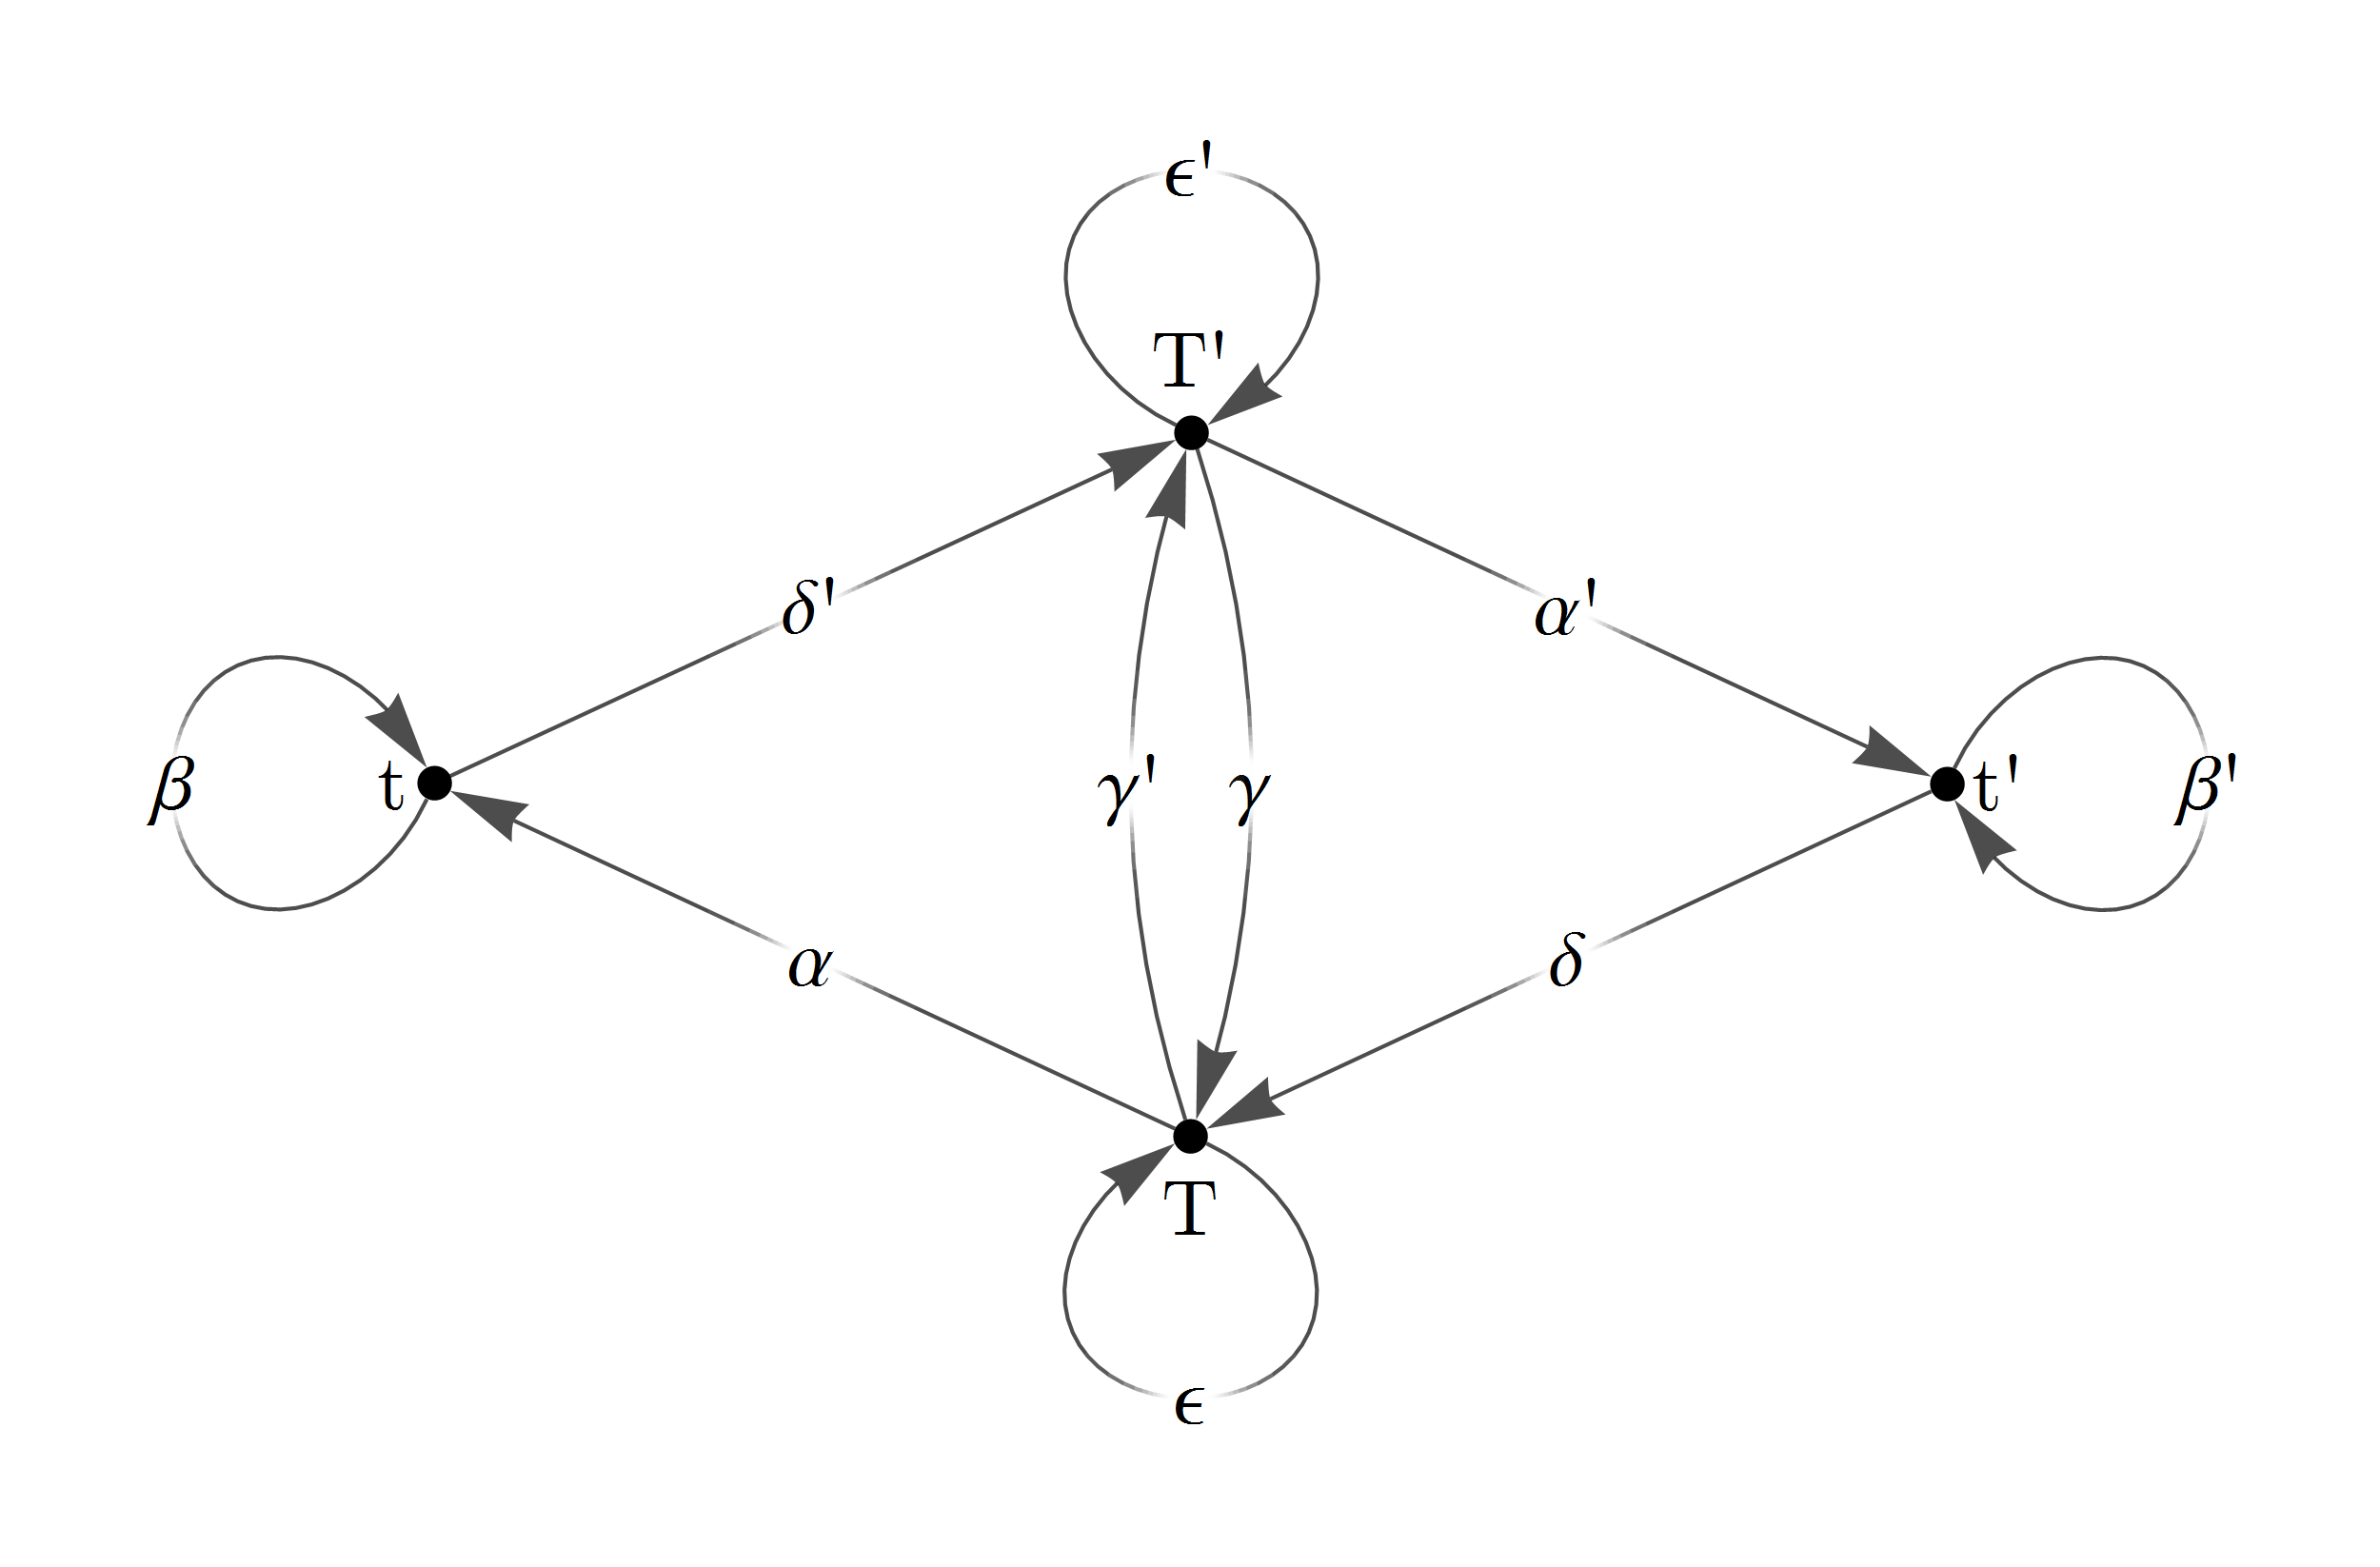
\includegraphics[width=\textwidth]{UpDownGraph}
\caption{A directed graph, or finite automaton, for the generation of parent triangles from constituent triangles. Paths along the directed edges represent compositions of the mappings from Equations (\ref{eq:maps}). Infinite paths along the directed edges may generate Penrose tilings of the plane.}
\label{fig:UpDownGraph}
\end{figure}

Paths along this directed graph represent compositions of the mappings. This is what is involved under the Up process, defining a sequence of the mappings. A finite sequence of mappings will directly correspond to a finite subregion of a Penrose tiling. The generation of the tiling region from the sequence of mappings is the Down process. Think of the Up process as producing a tiling instruction manual, and the Down process as following these instructions to produce a tiling. 

The Down process can describe a tiling region from the Up sequence because the mappings explicitly describe the relationship among substitution triangles. Even though each mapping only directly describes the relationship between a constituent triangle and its parent, we have also determined the placement of the other constituent oriented Robinson triangles of that parent. Further, the substitution rules from Fig.\ref{fig:OrientedRob} explicitly described the substitutions of the other constituent triangles. With this in mind, we can see how the Down process generates tiling regions from the Up process instructions. Essentially, the sequence of mappings from the Up process describes a sequence of substitutions, the Down process preforms these substitutions.

For an example of a finite sequence of the Up-Down process, consider the Up sequence from the graph path $\delta'\gamma\epsilon$ which defines the composition $\epsilon \circ \gamma \circ \delta'$. From the graph in Fig.\ref{fig:UpDownGraph} we can see that this Up sequence takes a \textbf{t} triangle and eventually embeds it into a \textbf{T} triangle. The Down process, given by this composition, then, will substitute that \textbf{T} triangle according to the composition sequence. This substitution ends once we've generated the initial \textbf{t} triangle. 


\begin{table}[H]
\begin{center}
\begin{tabular}{ccc}
\Large Up & & \Large Down\\
\raisebox{0px}{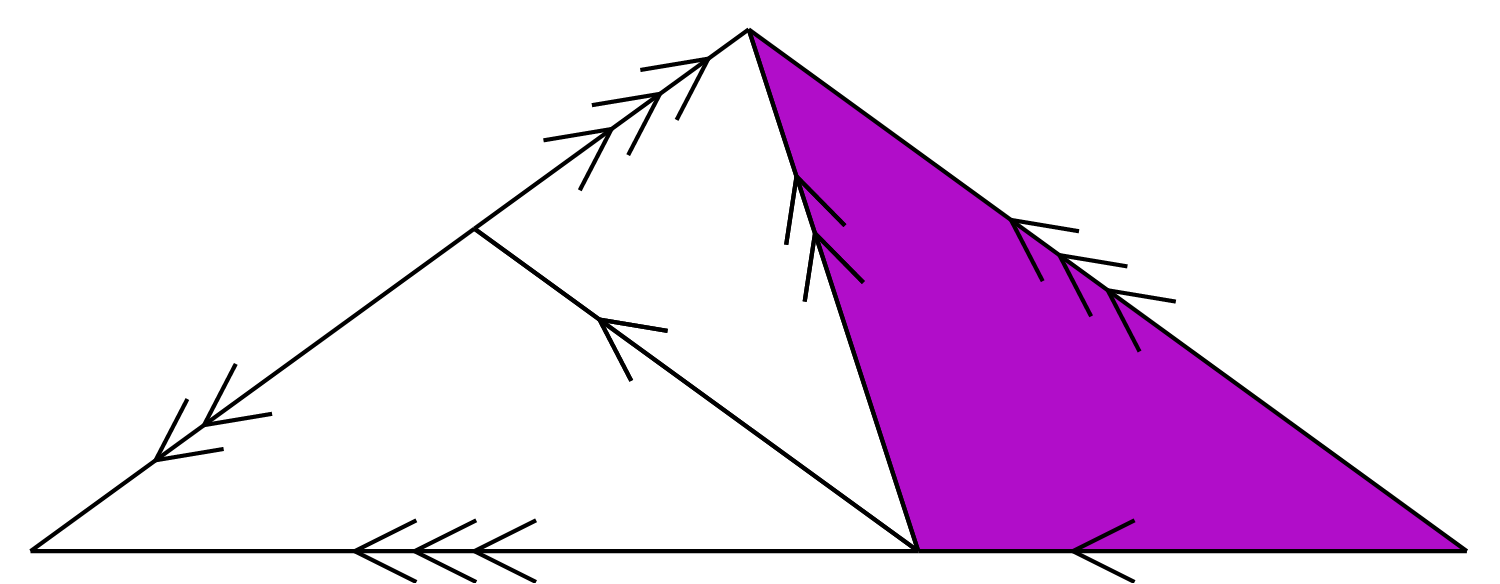
\includegraphics[width=0.3\textwidth]{Up4Left}} & \raisebox{20px}{\Large \textcolor{gray}{$ \rightarrow$}} & 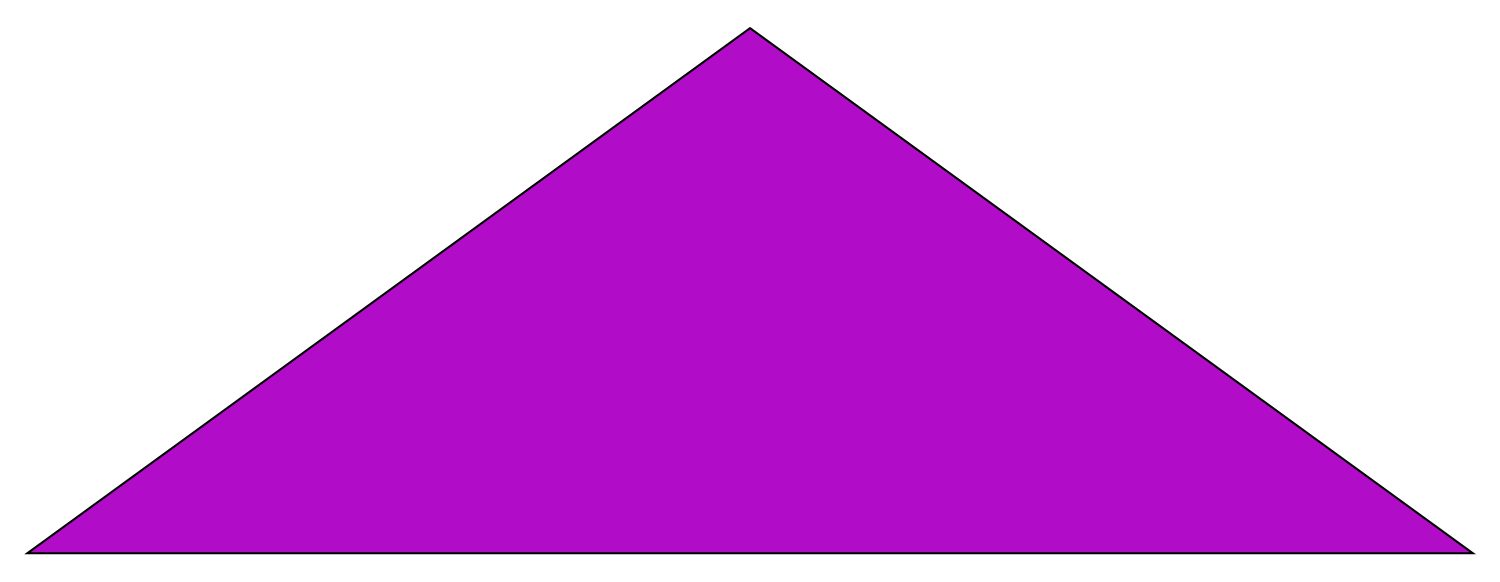
\includegraphics[width=0.6\textwidth]{Down4}\\
\Large $\uparrow$ $\epsilon$ & \hfill & $\downarrow$\\ 
\raisebox{0px}{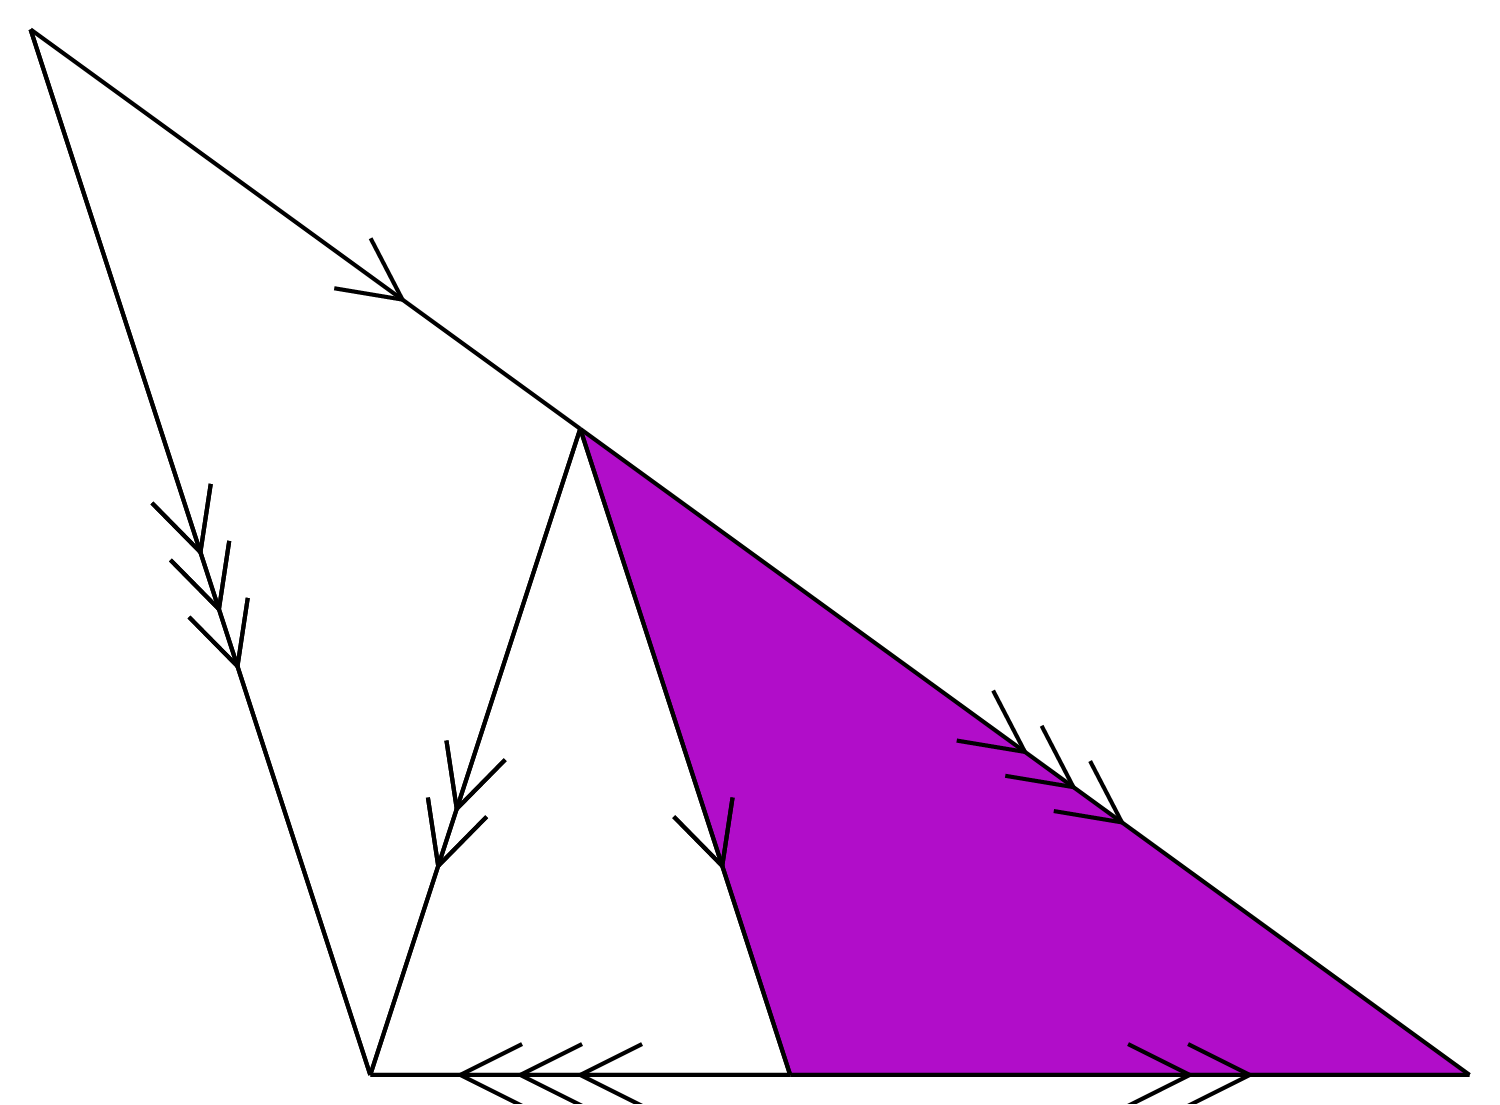
\includegraphics[width=0.3\textwidth]{Up3Left}} & \raisebox{30px}{\Large \textcolor{gray}{$ \rightarrow$}} & 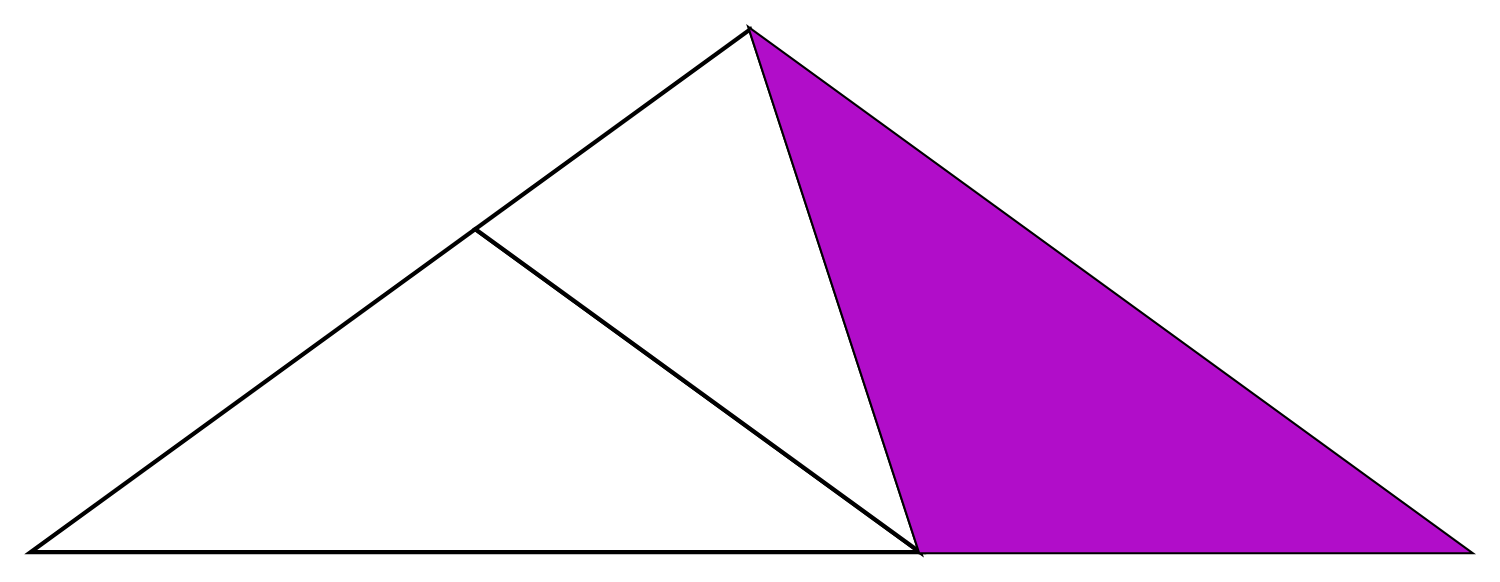
\includegraphics[width=0.6\textwidth]{Down3}\\
\Large $\uparrow$ $\gamma$ & \hfill & $\downarrow$\\ 
\raisebox{0px}{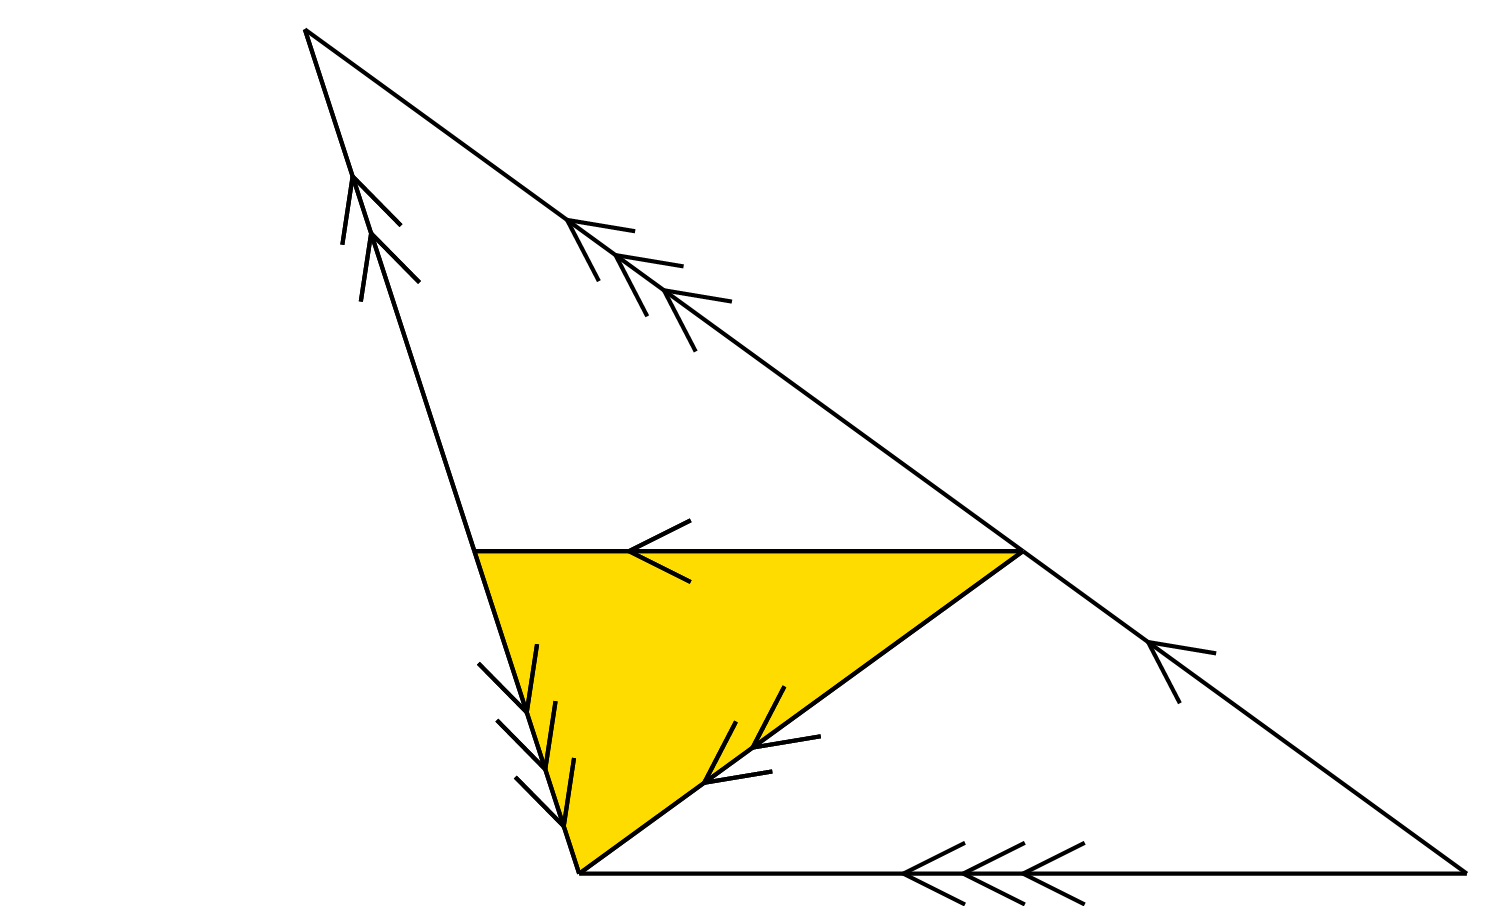
\includegraphics[width=0.4\textwidth]{Up2Left}} & \raisebox{30px}{\Large \textcolor{gray}{$ \rightarrow$}} & 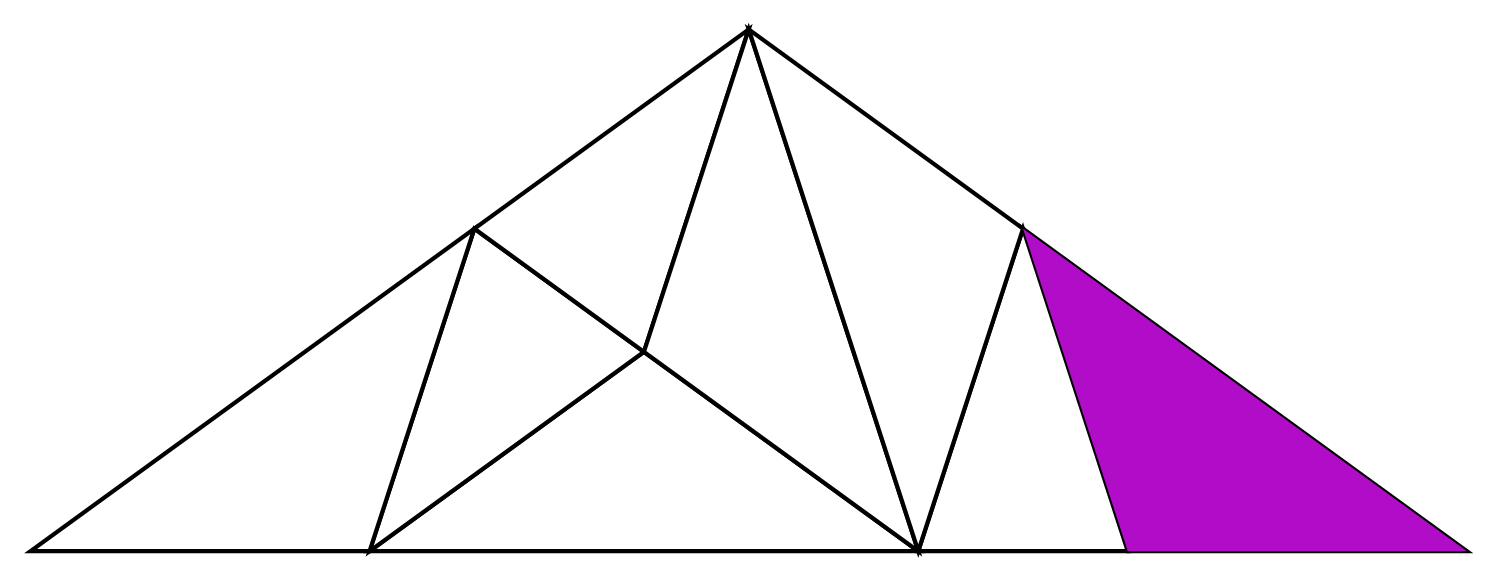
\includegraphics[width=0.6\textwidth]{Down2}\\
\Large $\uparrow$ $\delta'$ & \hfill & $\downarrow$\\ 
\raisebox{0px}{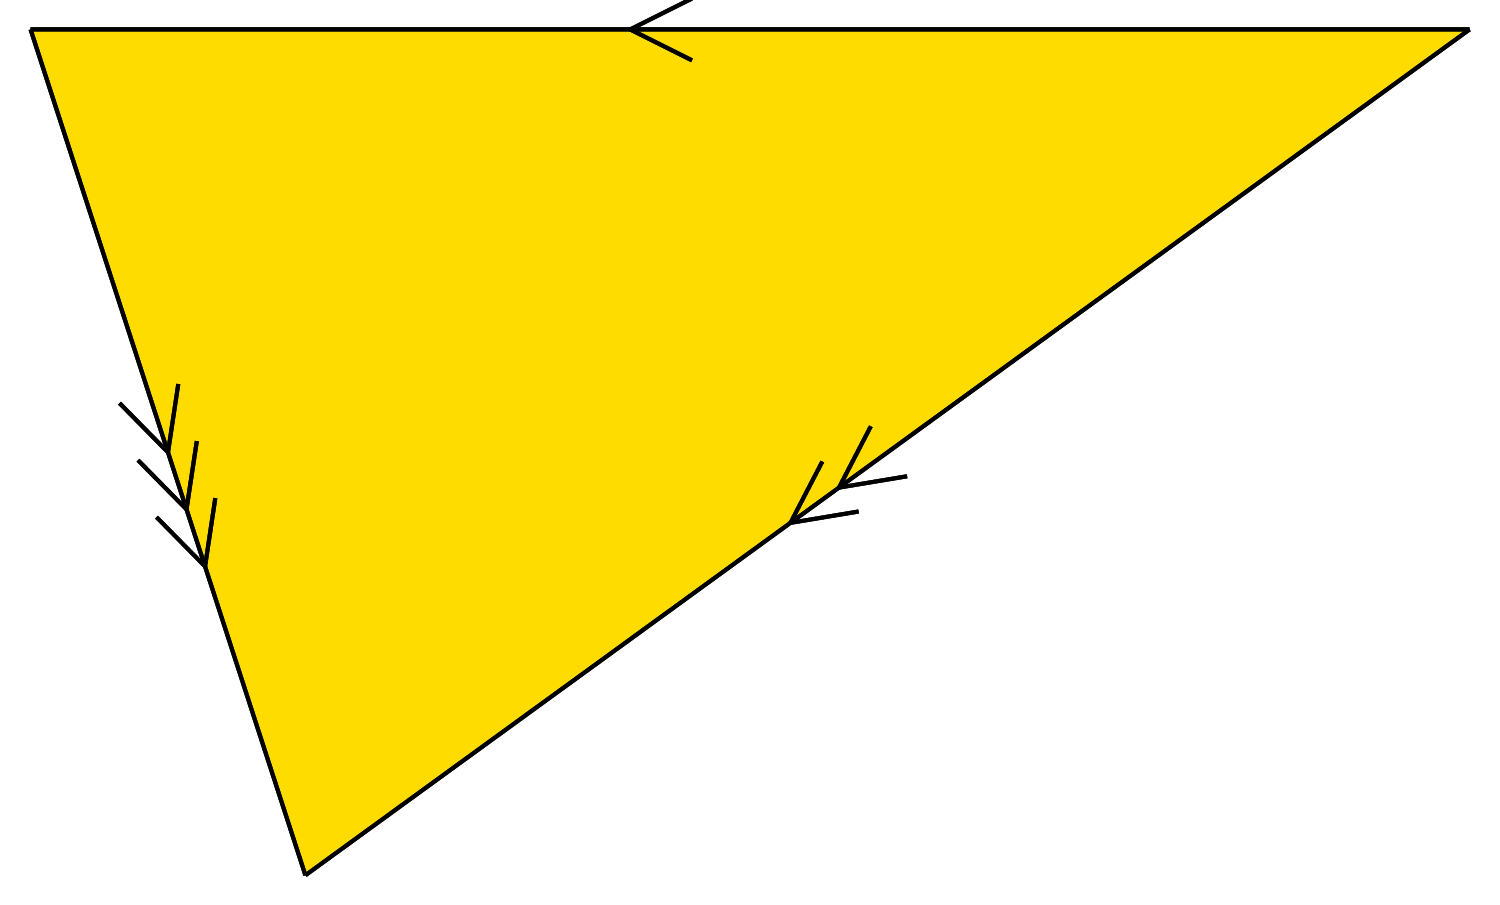
\includegraphics[width=0.3\textwidth]{Up1Left}} &\raisebox{30px}{\Large \textcolor{gray}{$ \rightarrow$}}& 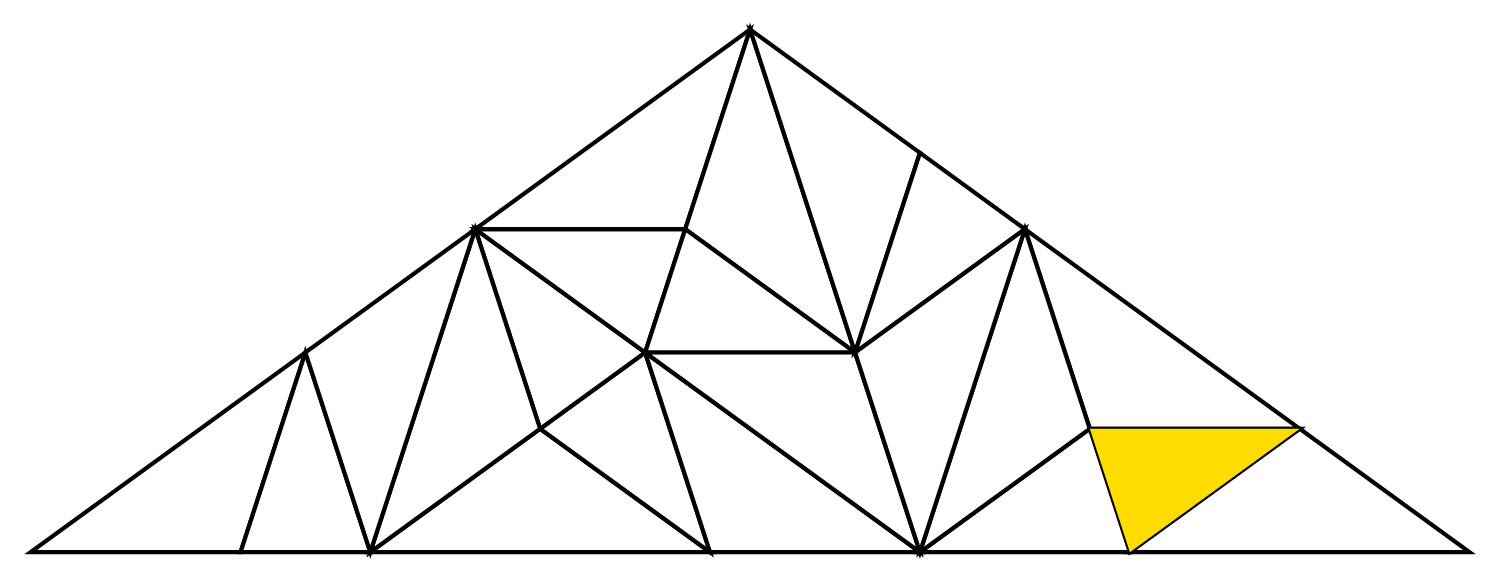
\includegraphics[width=0.6\textwidth]{Down1}\\
\end{tabular}
\end{center}
\captionof{figure}{A finite region generated by the Up-Down process. The Up sequence $\delta'\gamma\epsilon$ describes the mapping composition $\epsilon \circ \gamma \circ \delta'$. The Up process maps a \textbf{t} triangle to a \textbf{T} triangle. The Down process applies those substitutions on a \textbf{T} triangle to generate the initial \textbf{t} triangle.}

\end{table}


Infinite sequences of the Up-Down process, corresponding to infinite paths along the directed graph, will generate Penrose tilings of the plane, half-plane, or $\frac{\pi}{5}$-plane wedge, depending on the sequence. Generating $\frac{\pi}{5}$-plane wedges are the result of repeated mappings into thin Robinson triangles, this occurs when the limit of the sequence generates a thin Robinson triangle. Effectively, wedges are when the `top' of the Up-Down process is an infinite \textbf{t} or \textbf{t'} triangle, and the Down process infinitely substitutes into this. Of course, under infinite sequences, the Up-Down process will have no `top' triangle, but we can see that certain arbitrarily long sequences can generate an arbitrarily large thin Robinson triangle tiling, and as such the limit of this process is the Penrose tiling of an infinite $\frac{\pi}{5}$-plane wedge. This is not a problem, however, in generating Penrose tilings of the entire plane, because these plane wedges can be extended to tilings of the plane by reflection along their edges. Reflections on the sides of wedges is valid under the edge matching rules, to illustrate this with finite thin Robinson triangles see Fig.\ref{fig:WedgeWheel}.  Penrose plane tilings generated by $\frac{\pi}{5}$-plane wedge reflection will exhibit fivefold rotational symmetry centered at the point of the wedge. As we will discuss later, five-fold rotational symmetry is only possible in aperiodic tilings, so this is a remarkable feature of Penrose tilings generated from plane wedges. Similarly, half-plane tilings occur when the limit of the process is an arbitrarily large thick Robinson triangle. Half-plane tilings can also be extended to full plane tilings by reflection across the base.

\begin{figure}
\centering
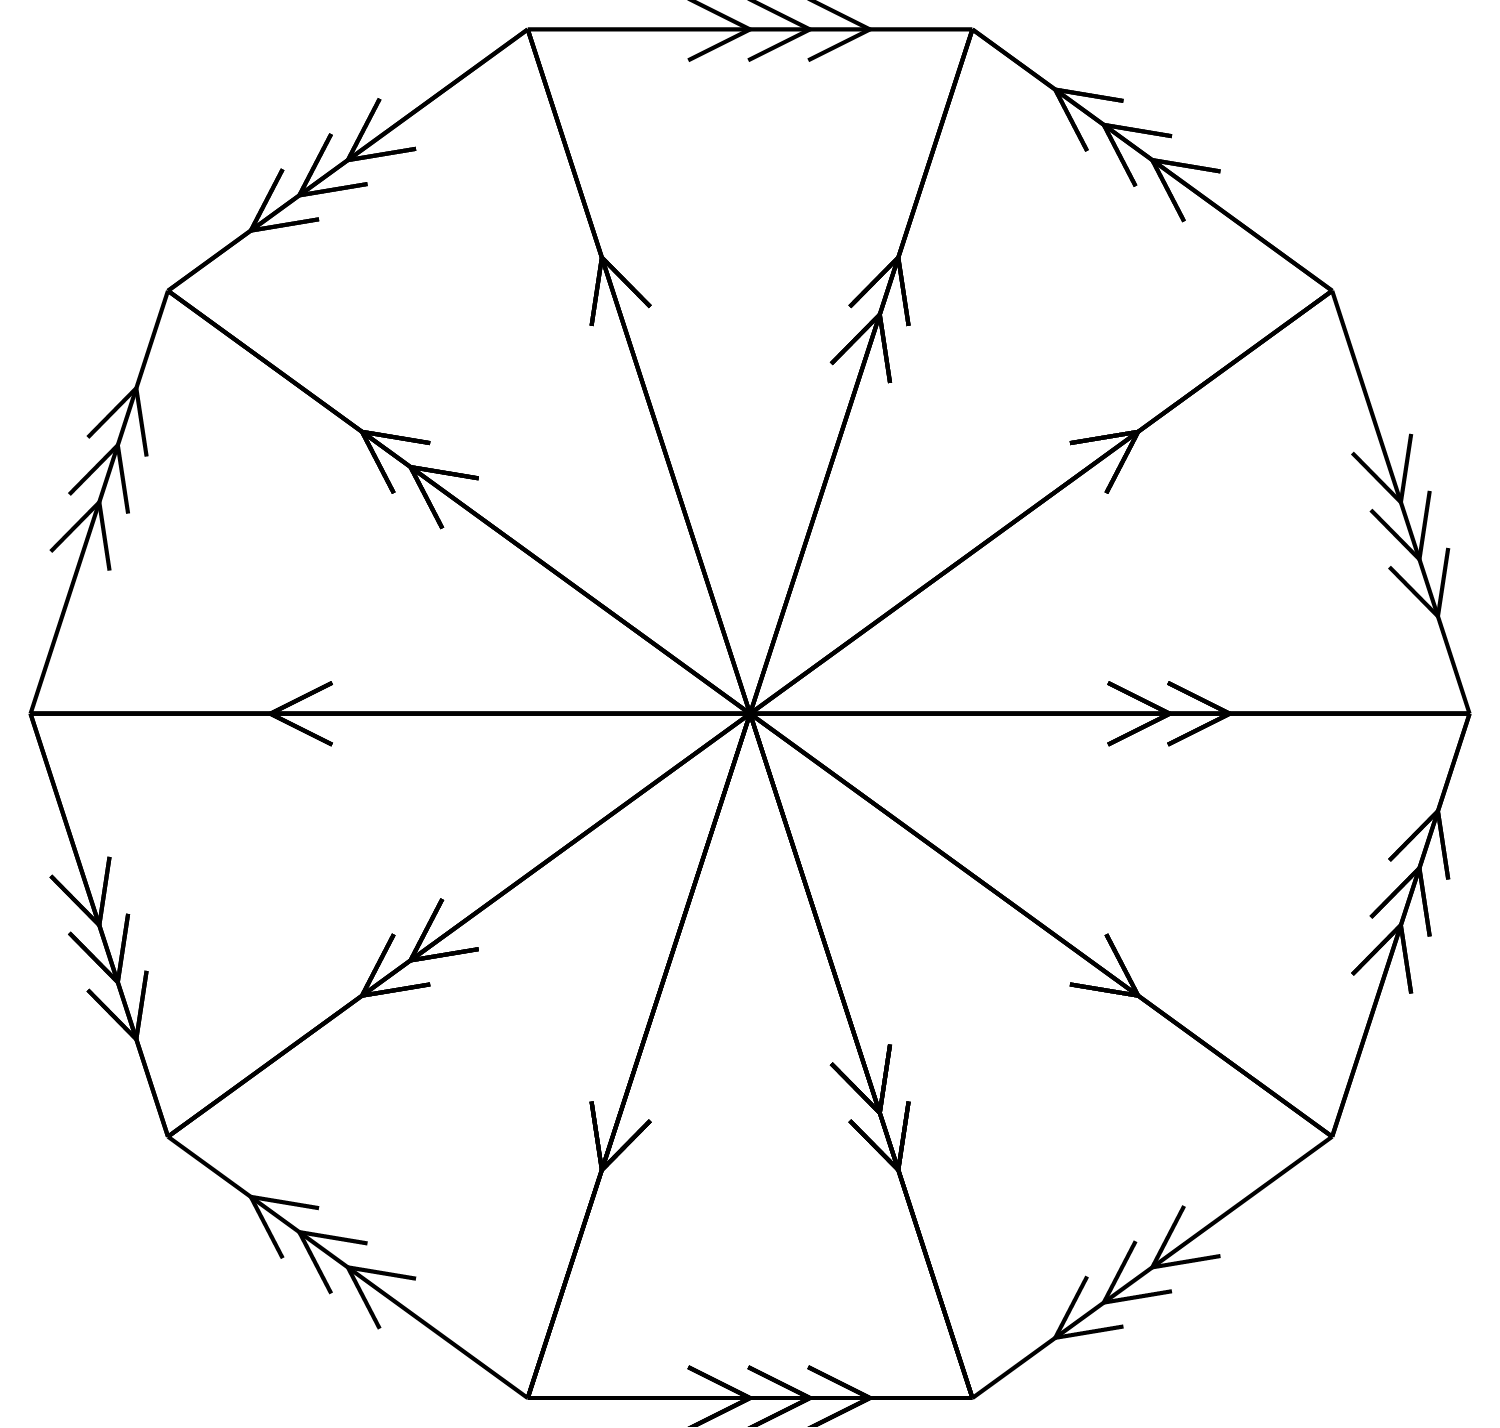
\includegraphics[width=0.5\textwidth]{WedgeWheel}
\caption{Reflection along sides of thin Robinson triangles produces valid arrangement of triangles under the edge matching rules. Demonstrated for finite triangles, this is also true for infinite  $\frac{\pi}{5}$-plane wedges. As such,  $\frac{\pi}{5}$-plane wedges can be extended to tilings of the entire plane under side reflection. Planes tiled in this way will exhibit fivefold rotational symmetry about the wedge point.}
\label{fig:WedgeWheel}
\end{figure}

\subsection{Penrose Tilings as Infinite Sequences}
We've seen how the Up-Down method generates Penrose tilings from infinite compositions of mappings. By describing these infinite compositions as sequences, we've alluded to an alternative representation of a Penrose tiling, as an infinite sequence of steps on the directed graph in Fig.\ref{fig:UpDownGraph}. 

\begin{mydef}
A \textbf{composition sequence}, $\rho$, is an infinite sequence of mappings which, under the Up-Down process, will take an elementary Robinson triangle to a Penrose tiling of the plane, half-plane, or $\frac{\pi}{5}$-plane wedge. Compositions sequences must correspond to infinite paths on the graph in Fig.\ref{fig:UpDownGraph}.
\end{mydef}

\begin{mylem}
Every composition sequence generates a Penrose tiling of a plane, half-plane, or $\frac{\pi}{5}$-plane wedge.
\end{mylem}

\begin{proof}
This follows directly from the Up-Down method.
\end{proof}

By the above lemma, we see that every composition sequence generates a Penrose tiling. However, Penrose tilings are not unique to a composition sequence.

\begin{mylem}
A Penrose tiling is generated by infinitely many composition sequences.
\end{mylem}

\begin{proof}
Consider a Penrose tiling, $\mathcal{T}$.\\
$\mathcal{T}$ is composed of infinitely many individual tiles.\\
By the Up-Down method, each tile can generate $\mathcal{T}$ by a unique composition sequence.\\
$\therefore$ There are infinitely many composition sequences which generate $\mathcal{T}$.
\end{proof}

We've now shown that while all composition sequences correspond to a Penrose tiling, this relationship isn't one-to-one. That is, we see that infinitely many sequences generate the same Penrose tiling. What determines whether the same Penrose tiling is generated by two different sequences?

\begin{mydef}
Two composition sequences, $\rho_1$ and $\rho_2$, are said to be \textbf{cofinal} if they agree after finitely many terms.
\end{mydef}

\begin{mythm}
Two composition sequences generate the same Penrose tiling if and only if they are cofinal.
\end{mythm}

\begin{proof}
Let $\rho_1$ and $\rho_2$ be composition sequences defining $\mathcal{T}_1$ and $\mathcal{T}_2$ respectively. \\[10pt]
If $\rho_1 = \rho_2$ then $\mathcal{T}_1 = \mathcal{T}_2$, and they are trivially cofinal.\\[10pt]
If $\rho_1$ and $\rho_2$ are cofinal, then, after, $n$, finitely many terms, the sequences agree.\\
Consider composition sequence, $\rho^*$, which begins where $\rho_1$ and $\rho_2$ agree.\\
$\rho^*$ defines a Penrose tiling  $\mathcal{T}^*$.\\
This implies that, at some hierarchal level, level $n$ in the Up process, $\rho_1$ and $\rho_2$ begin describing the same tiling.\\
By the Up-Down process, substitution is uniquely defined.\\
Therefore, $\mathcal{T}^*$ uniquely determines $\mathcal{T}_1$ after $n$ substitutions.\\
Likewise, $\mathcal{T}^*$ uniquely determines $\mathcal{T}_2$ after $n$ substitutions.\\
$\therefore$ $\mathcal{T}_1 = \mathcal{T}_2$ if  $\rho_1$ and $\rho_2$ are cofinal.\\[10pt]
Conversely, suppose $\mathcal{T}_1 = \mathcal{T}_2$ and call this tiling $\mathcal{T}$. \\
Let $\rho_1$ begin with the tile  ${\rho_1}_0$.\\
Let $\rho_2$ begin with the tile ${\rho_2}_0$.\\
Then ${\rho_1}_0$ and ${\rho_2}_0$ both belong to $\mathcal{T}$.\\
The distance between ${\rho_1}_0$ and ${\rho_2}_0$ is therefore finite.\\
Then at some hierarchal level, after finite $n$ in the Up process, a single tile will contain both ${\rho_1}_0$ and ${\rho_2}_0$.\\
$\rho_1$ and $\rho_2$ will agree after this level.\\
$\therefore$ $\rho_1$ and $\rho_2$ are cofinal if $\mathcal{T}_1$ and $\mathcal{T}_2$.
\end{proof}

We now see that all cofinal sequences are related to each other by the unique Penrose tiling they generate. This defines an equivalence class.

\begin{mydef}
Cofinality of composition sequences defines an equivalence relation on the set of composition sequences. Equivalence classes of cofinal sequences are called \textbf{families}.
\end{mydef}

Further, we can consider a function, $C(\rho)$, which takes a composition sequence and returns its parent sequence. In other words, if $\rho$ defines a Penrose tiling, $C(\rho)$ defines the tiling before the previous substitution. 

\begin{mylem}
$\rho$ and $\rho'$ are cofinal if and only if $C(\rho)$ and $C(\rho')$ are cofinal.
\end{mylem}

\begin{proof}
Let 
\begin{equation*}\begin{split}
\rho=\{\rho_0,\rho_1,\rho_2,\rho_3,\mathellipsis\}\\
\rho'=\{\rho'_0,\rho'_1,\rho'_2,\rho'_3,\mathellipsis\}
\end{split}
\end{equation*}\\
Then 
\begin{equation*}
\begin{split}
C(\rho)=\{\rho_1,\rho_2,\rho_3,\mathellipsis\}\\
C(\rho')=\{\rho'_1,\rho'_2,\rho'_3,\mathellipsis\}
\end{split}
\end{equation*}\\
By definition of cofinality and inspection, $\rho$ and $\rho'$ are cofinal if and only if $C(\rho)$ and $C(\rho')$ are cofinal.
\end{proof}

Further, $C(\rho)$ allows us to address a common misconception regarding Penrose tilings. When looking at a graphical representation of a tiling, especially when considering their construction by substitution, it is easy to assume that the Penrose tiling is self-similar. We can easily show this is not the case in general.

\begin{mylem}
Penrose tilings are, in general, not self-similar.
\end{mylem}

\begin{proof}
Consider a Penrose tiling, $\mathcal{T}$.\\
$\mathcal{T}$ is given by composition sequence $\rho$.\\
In general, $C(\rho)\neq\rho$.\\
$\therefore$ Penrose tilings are not self-similar.
\end{proof}

However, we arrive at something of a veridical paradox here. We've just shown that Penrose tilings are not self-similar. However, we also know that, trivially, $\rho$ and $C(\rho)$ are cofinite. Therefore, we see that $\rho$ and $C(\rho)$ define the same Penrose tiling. That is, substitution of a Penrose tiling will map the tiling back to itself, but this will not be self-similar. 

Finally, we are ready to see the greatest benefit to considering Penrose tilings as equivalence classes of composition sequences.

\begin{mythm}
There are uncountably many Penrose tilings.
\end{mythm}

\begin{proof}
Every Penrose tiling is uniquely determined by a family of cofinal composition sequences.\\
By Cantor's Diagonalization Argument, if there were countably many Penrose tilings then we could construct a countable list of infinite sequences, with one sequence from each family.\\
However, by considering infinite paths on the directed graph or recalling the proof of the uncountability of real numbers, we see that given such a countable list we can always construct a composition sequence that is not a member of that list.\\
Therefore, a countable list of composition sequence families will always be incomplete.\\
Therefore, there are uncountably many composition sequence families.\\
$\therefore$ there are uncountably many Penrose tilings by Cantor's Diagonalization.
\end{proof}

\end{document}